\documentclass[11pt, a4paper ]{article}

\usepackage[utf8]{inputenc}
\usepackage[T1]{fontenc}
\usepackage[top=2.5cm, bottom=2.5cm, left=2.5cm, right=2.5cm]{geometry}
\usepackage[francais]{babel}
\usepackage{wrapfig}
\usepackage{graphicx}
\usepackage{makeidx}
\usepackage{url}
\usepackage{tabularx}
\usepackage{setspace}

\setmainfont{Arial}

\makeindex
%\usepackage{fontspec}
%\setmainfont{Arial}

\title{Mémoire Titre qui en jette grave}
\author{Julien Prugne 108287}
\date{Avril 2014 à Octobre 2014}

% new page for every section
\let\stdsection\section
\renewcommand\section{\newpage\stdsection}

\begin{document}


	\maketitle
	\tableofcontents

	% TODO: à la toute fin
\begin{spacing}{1.5}
	\section{Introduction} %3 pages

	% TODO: avant intro et conclusion
	% récolter assez d'info
	%\chapter{présentation entreprise et mise en context : titre personalisé} % 25 pages


	\section{Présentation de l'entreprise: titre personnalisé} % 15 pages trouver un meilleur titre

			%intro de partie
DOM Element Inc. est une startup Montréalaise.

Une startup\cite{theseStartup} est une jeune entreprise. C'est une structure ayant pour but de défricher un nouveau pan de l'économie. Il s'agit d'entreprise généralement incarnée par leur(s) créateur(s) et fondant son modèle économique sur l'innovation. Cette capacité d'innovation est l'ADN des startups.

Dans un premier temps, l'entreprise en elle-même n'est qu'une structure légale offrant une interface avec des structures ayant la capacité de financer l’essor du projet. En effet, les plans d'affaire de ce genre d'entreprise prévoient généralement des pertes sur les premiers temps de son développement, voir pour l'intégralité de son existence. Cela peut sembler incohérent au premier abord mais un écosystème s'est créé autour des startups. Composé de riches particuliers\footnote{Bussiness Angel}, de groupes financiers gérant un fond privé\footnote{venture capital} ou encore de concours entrepreneurial, cet écosystème crée un flux entrant de capitaux dans cette économie. Ces derniers ont généralement pour objectif de rentabiliser leurs investissements lors de la vente ou de la capitalisation boursière de la startup. Les montants en jeux sont considérables; les investissements ou les ventes de telles sociétés se chiffrent en dizaine, centaine de milliers de dollars, certain cas allant jusqu'à plusieurs milliards de dollars.

Les perspectives de ces marchés semblent extrêmement intéressantes mais il faut pondérer ces assertions par le taux d'échec impressionnant des startups. En effet, au bout de 4 ans seul cinquante pour-cent des startups semblent encore en activité. Ce pourcentage chute drastiquement au bout de dix ans puisque seul vingt-neuf pour-cent d'entre elles seront encore en activité.
Beaucoup de chiffres pourraient être cités mais aux vues de l'aspect encore sauvage de cette économie, il est peu probable que les chiffres reflètent la réalité tumultueuse de ces chasseurs d'or de nouvelle génération.
Toute fois, les statistiques semblent s'accorder sur une tendance générale: le taux d'échec des startups est colossal mais les réussites sont spectaculaires.

La majorité arrêtera par manque de moyens financiers empêchant de mener le projet à maturité. Un certain nombre vivra quelques années au frais du venture capitalism, une petite portion sera achetée par de gros groupes\footnote{skype par microsoft pour 8,5 milliards de dollars, instagram par facebook pour 1 milliard de dollars, etc.} et enfin, une infime partie deviendra de larges entreprises\footnote{exemple: facebook, twitter, Google,...} après capitalisation.

\begin{center}
	\begin{tabular}{l*{1}{c}}
		Années  & Taux d'échec\\
		\hline
		1 & 25\% \\
		4 & 50\% \\
		7 & 63\% \\
		10 & 71\% \\
	\end{tabular}\cite{statEchecStartup}
\end{center}

Attention, toutes les jeunes entreprises ne sont pas des startups. Une startup est caractérisée par sa capacité à générer de la croissance et de l'innovation rapidement. Le taux de croissance hebdomadaire du nombre d'utilisateurs est l'indicateur le plus révélateur de la bonne santé d'une startup.

\begin{quote}
	[...]

	Commençons par faire une distinction qui est souvent ignorée: toutes les compagnies financées ne sont pas des startups. Des millions de compagnies sont créées chaque année aux États-Unis. Seule une petite fraction de ces entreprises sont des startups. La plupart sont des services commerciaux - restaurants, coiffeurs, plombier, etc. Ce ne sont pas des startups sauf dans quelques cas particuliers. Un salon de coiffure n'est pas prévu pour une croissance exponentielle. Contrairement à un moteur de recherche.

	[...]


	\caption{Paul Graham, \emph{Startup = Growth\cite{startupGrowth}}}
\end{quote}

Une startup est donc avant tout un projet soutenu par une équipe passionnée et persuadée de la pertinence de leur solution et de sa capacité à générer de la croissance. Nous, chez HappyBox nous voulons rendre la création web accessible à tous.

		% présentation générale HappyboxCMS = intro plan d'affaire
		%	historique à étoffer
		\subsection{L'équipe} %2 pages max
DOM Element étant une très petite structure composée de ses deux co-fondateurs: Danny Coulombe et Guillaume Lagacé, de deux actionnaires minoritaires chargés de la communication: Brendan Shera-shriar et Brendan Tully-Walsh et de un ou deux stagiaires selon l'époque: François Lacroix-Durant et moi même.
\begin{center}
	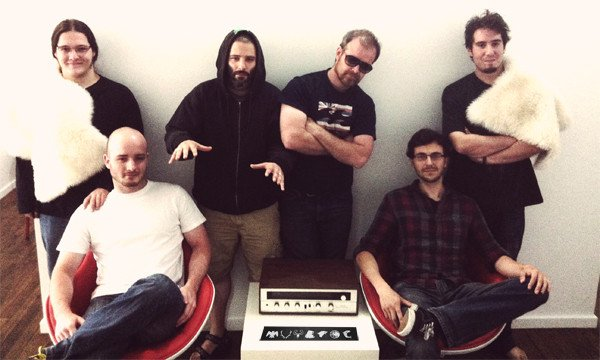
\includegraphics[width=\textwidth]{images/team/team.jpg}

	 De gauche à droite: François Lacroix-Durant, Danny Coulombe, Brendan Sera-Shriar, Brendan Tully Walsh, Guillaume Lagacé et Julien Prugne.
\end{center}

\paragraph{}
	Guillaume Lagacé a le rôle de \emph{CEO}, Chief Executif Officer ou Président Directeur Générale en français, Il a pour responsabilité de mettre en place la structure globale de l'entreprise.
	Ses tâches incluent:

		\begin{itemize}
			\item
				Relations avec les financiers
			\item
				Définition de la stratégie d'entreprise.
			\item
				Coordination de l'équipe
			\item
				Entretien des relations d'affaires
		\end{itemize}

\paragraph{}
Danny Coulombe est le \emph{CTO}, Chief Technolgy Officer ou Directeure de la Technologie en français. Il est le développeur principal d'HappyBox CMS. Il est responsable des orientations technologiques et de la gouvernance du développement du produit.

	Ses tâches incluent:

		\begin{itemize}

			\item
				Développement \emph{Full Stack\footnote{Expression en vogue désignant un développeur web alliant à la fois des compétences de développement front-end et back-end ainsi que des compétences en administration systèmes. Il s'agit d'un profil complet capable de créer, déployer et maintenir une application web dans sa totalité.}}
			\item
				Design interface utilisateur
			\item
				Optimisation d'expérience utilisateur
			\item
				Prototypage

		\end{itemize}



\paragraph{} %brendans
	\emph{The Brendans} est une agence de communication digitale anglophone Montréalaise. Ses deux membres fondateurs, Brendan Shera-Shriar et Brendan Tully-Walsh, sont actuellement actionnaires à hauteur de 2\% de Dom Element Inc. Ils ont pour mission, avec leur équipe, de promouvoir HappyBox CMS sur les réseaux sociaux, de créer et d'entretenir l'image du produit.
	C'est un élément fondamental de l'accès au web. Seules les compagnies ayant une bonne visibilité auprès de leur cible et entretenant de bons rapports avec leurs clients, semblent émergées.

		\subsection{Historique DOM Element Inc.}
%%%%%%%%%% TODO: INTEGRER LE RESEAUX ET LES CONCOURS ICITTE %%%%%%%%%%%%%%%%%
% Avril 2013 Fondation Montréal Inc. (12 000)
% Juin 2013 Jeunes Promoteurs (18 000)
% Février 2014 SDEVM (10 000)

\paragraph{}
\emph{HappyBox CMS}, a vu le jour en Octobre 2012, lorsque Guillaume Lagacé et Danny Coulombe, fondateurs de l'agence digitale \emph{WebRight\footnote{\url{http://webright.ca/fr}}} décident d'élaborer un moteur de création web alliant simplicité d'utilisation, technologie de pointe et créativité.

\paragraph{}
Pour arriver à leurs fins, ils enregistrent la société \emph{DOM Element Incorporated} le 23 Octobre 2012 auprès du registraire des entreprises du Québec via la société \emph{Dufourd, Dion Avocats}. Les droits du produit HappyBox CMS sont cédés à \emph{DOM Element Inc}, Danny et Guillaume se partagent alors la compagnie en deux parts égales, leur conférant un pouvoir décisionnel commun et équivalent au sein de l'entreprise.

\paragraph{}
Durant les deux mois suivants, les efforts s'orientent sur le développement du projet \emph{HappyBox CMS}.
En décembre 2013, l'équipe rencontre Brendan Shera-Shriar et Brendan Tully-Walsh, co-fondateurs de l'agence de communication digitale \emph{The Brendans} qui deviendront, le 15 mai 2013 des actionnaires et membres exécutifs de DOM Element Incorporated en échange de leur expertise en terme de communication et d'acquisition de clientèle.


\paragraph{}
Ce même mois de mai 2013, HappyBox CMS, nom de produit approuvé plus tôt en février, est sélectionné pour faire partie de la \emph{cohorte de la fondation Montreal Inc.} et recevra une bourse de \$12000. Bourse qui sera utilisée pour le financement du développement et de la communication autour du produit.

%%%%%%%%%%%%%%%%%%%%%%%%%%%%%%%%%%%%%%%
%%%%%% PARLER DES LOCAUX  + choix model freemium %%%%%%%
%%%%%%%%%%%%%%%%%%%%%%%%%%%%%%%%%%%%%%%

\paragraph{}
En juin 2013, François Lacroix-Durant et moi-même intégrons les rangs de DOM Element Inc., respectivement en tant qu'intégrateur web et administrateur systèmes. A la même période HappyBox reçoit une bourse de  \$18,000 grâce au programme \emph{Jeunes Entrepreneurs} organisé par la société de développement économique de Ville-Marie.

\paragraph{} %%%% raconter l'été 2013
Durant l'été 2013, nous nous installons dans un loft partagé avec les Brendans situé dans le vieux port de Montréal. Nous avons, François, Guillaume, Danny et moi-même passé l'été à développer le produit, les infrastructures nécessaires pour accueillir HappyBox CMS et le modèle freemium actuellement en vigueur sur HappyBox CMS.


\paragraph{}
À l'automne 2013, le service en ligne HappyBox CMS ouvre ses portes pour une phase d'alpha privé comptant déjà une centaine d'utilisateurs. Principalement des développeurs, des agences de Marketing Montréalaises ainsi que l'entreprise Maaco\footnote{Maaco est une des plus grandes chaînes de peinture et de réparation de véhicules d'Amérique du nord.}.

\paragraph{}
Le 19 Novembre 2013, HappyBox CMS se classe second au grand concours entrepreneurial \emph{Prix Montreal Inc}..
%%%%%% TODO: manquant décembre 2013 à maintenant %%%%%%%

\paragraph{}
En février 2014, Dom Element reçoit une nouvelle bourse de \$10,000 de la part de la Société de développement économique de Ville-Marie.
%%%%%% FIN                                       %%%%%%%

			\subsection{Plan d'affaire: le modèle freemium} % 11 pages
% Là faut charger! cible tout du long

\paragraph{}
% intro model freemium
Le \emph{modèle freemium\index{freemium!modèle}} est un type de plan d'affaire. Le mot \emph{freemium} est la contraction de deux termes anglophones : \emph{free} et \emph{premium}. Ce modèle économique se voue à proposer un produit ou un service gratuitement à la majorité de ses utilisateurs afin que tous puissent accéder librement au produit. En plus de cette offre gratuite, il est proposé à l'utilisateur une offre dite premium qui , elle, est payante et transforme une partie des utilisateurs en clients générateurs de revenu. La minorité des utilisateurs payant le service premium financera la plate-forme pour l'intégralité de ses usagers.


% présentation détaillée
\paragraph{} % offre gratuite
L'offre gratuite ne peut pas et ne doit pas être une version d'essai inutilisable sans recourir au service premium. Ce doit être un produit répondant à un besoin de l'utilisateur ou lui offrant un produit ou un service dont il aurait envie. Cette base d'utilisateurs ne payant pas est vitale au bon fonctionnement de cette stratégie d'affaire.

\subparagraph{} % exemple offre gratuite Skype + Farmville
L'exemple le plus frappant est sûrement Skype, ce dernier propose un service de voix et de vidéo sur internet entièrement gratuit pour ses utilisateurs. La majorité des utilisateurs ne paieront jamais pour utiliser un service optionnel puisqu'il leur est permis gratuitement et de manière illimitée de faire des visioconférences internationales.

Un autre exemple populaire pourrait être les jeux de gestion sur Facebook type \emph{Farmville\footnote{Un des soixante-sept titres de la compagnie Zynga étant accessible via Facebook}} proposant gratuitement des jeux complets, avec des mécaniques basées sur l'interaction sociale avec le réseau du(de la) joueur(joueuse\footnote{La cible de prédilection de ces compagnies n'est pas la même que les autres compagnies de jeux vidéo, les adolescents de 14 à 24 ans, car ces derniers ont du temps mais n'ont peu voir pas d'argent ni de carte de crédit, ils constitueront la masse des joueurs offrant la visibilité nécessaire au jeu. Le véritable marché cible se situe auprès des ménagères d'âge moyen, femmes au foyer qui semblent être les véritables payeuses des jeux sociaux.}) rendant le produit addictif pour ses utilisateurs.

\paragraph{} % offre payante
Il est évident que seule une offre gratuite ne peut suffire à garantir les revenus nécessaires au fonctionnement de l'entreprise. C'est là qu'intervient l'offre premium. C'est un complément à l'offre gratuite, une amélioration significative de l’expérience utilisateur mais théoriquement sans la dénaturer. Cette offre surclassée doit permettre de financer l'offre gratuite ou compenser dans un premier temps au maximum les coûts de l'offre gratuite.
\subparagraph{}
L'offre premium peut porter sur différents type de services mais doit toujours être en adéquation avec l'offre gratuite. Dans les faits, la définition de l'offre premium étant intimement liée au produit, il est impossible de définir un modèle unique et applicable à tous types d'affaire. On remarque tout de même que de grandes tendances semblent se dessiner et cela vient de la concurrence importante sur les marchés porteurs de freemium. Ainsi beaucoup semblent adopter la même ligne d'affaire et offrir des services similaires du moment qu'ils proposent des offres similaires. La copie des plans d'affaires de société en pleine expansion est une stratégie vieille comme le monde.

\subparagraph{} % L'exemple de Skype et Farmville

On ne compte plus le nombre de jeux gratuits sur Facebook offrant des achats \emph{in app} ne coupant pas l'expérience de jeu et permettant d’accélérer la progression des joueurs. Ce qui évite ainsi d'avoir à subir la difficulté de l'expérience d'un jeu optimisé pour la conversion des utilisateurs de l'offre gratuite en utilisateurs payeurs. L'achat sera donc le plus souvent impulsif pour gagner du temps de jeu afin de dépasser ses \emph{amis Facebook} ou tout simplement de pouvoir continuer à jouer. Car dans ce genre d'application, la tendance semble être à la limitation du nombre d'action à effectuer dans un temps donné, le tout avec une possibilité de paiement pour éviter d'attendre\footnote{Il s'agit de coupe-file numérique.}. Au moment où ces lignes sont écrites \emph{Farmville 2 développé par Zynga} compte dix millions d'utilisateurs mensuels mais seul 3\% de ces utilisateurs paieront une offre premium.


La cible de ces produits sont des amateurs de jeux néophytes en terme de pratique vidéo-ludique qui ne se rendront pas compte que le rapport divertissement/coût est un des plus mauvais sur le marché.

\subsubparagraph{}
Les applications d'écoute de musique\footnote{Spotify, Deezer, Groove Shark, Google Music, ...} proposent généralement une offre gratuite incluant publicité durant les temps d'attente, des limitations sur le nombre de morceaux écoutables ainsi que le nombre d'écoute d'un même morceau.
Le paiement d'un abonnement supprime à la fois la publicité et la limitation d'écoute ainsi que l'ajout de fonctionnalités\footnote{Fichier musicaux de meilleure qualité, vente ou location de titre numérique} comme par exemple, une synchronisation des fichiers sur un appareil afin d'offrir un accès hors ligne. Plusieurs types d'offre payante pourront ainsi être proposés.

%%% offre premium spotify %%%

\begin{center}
	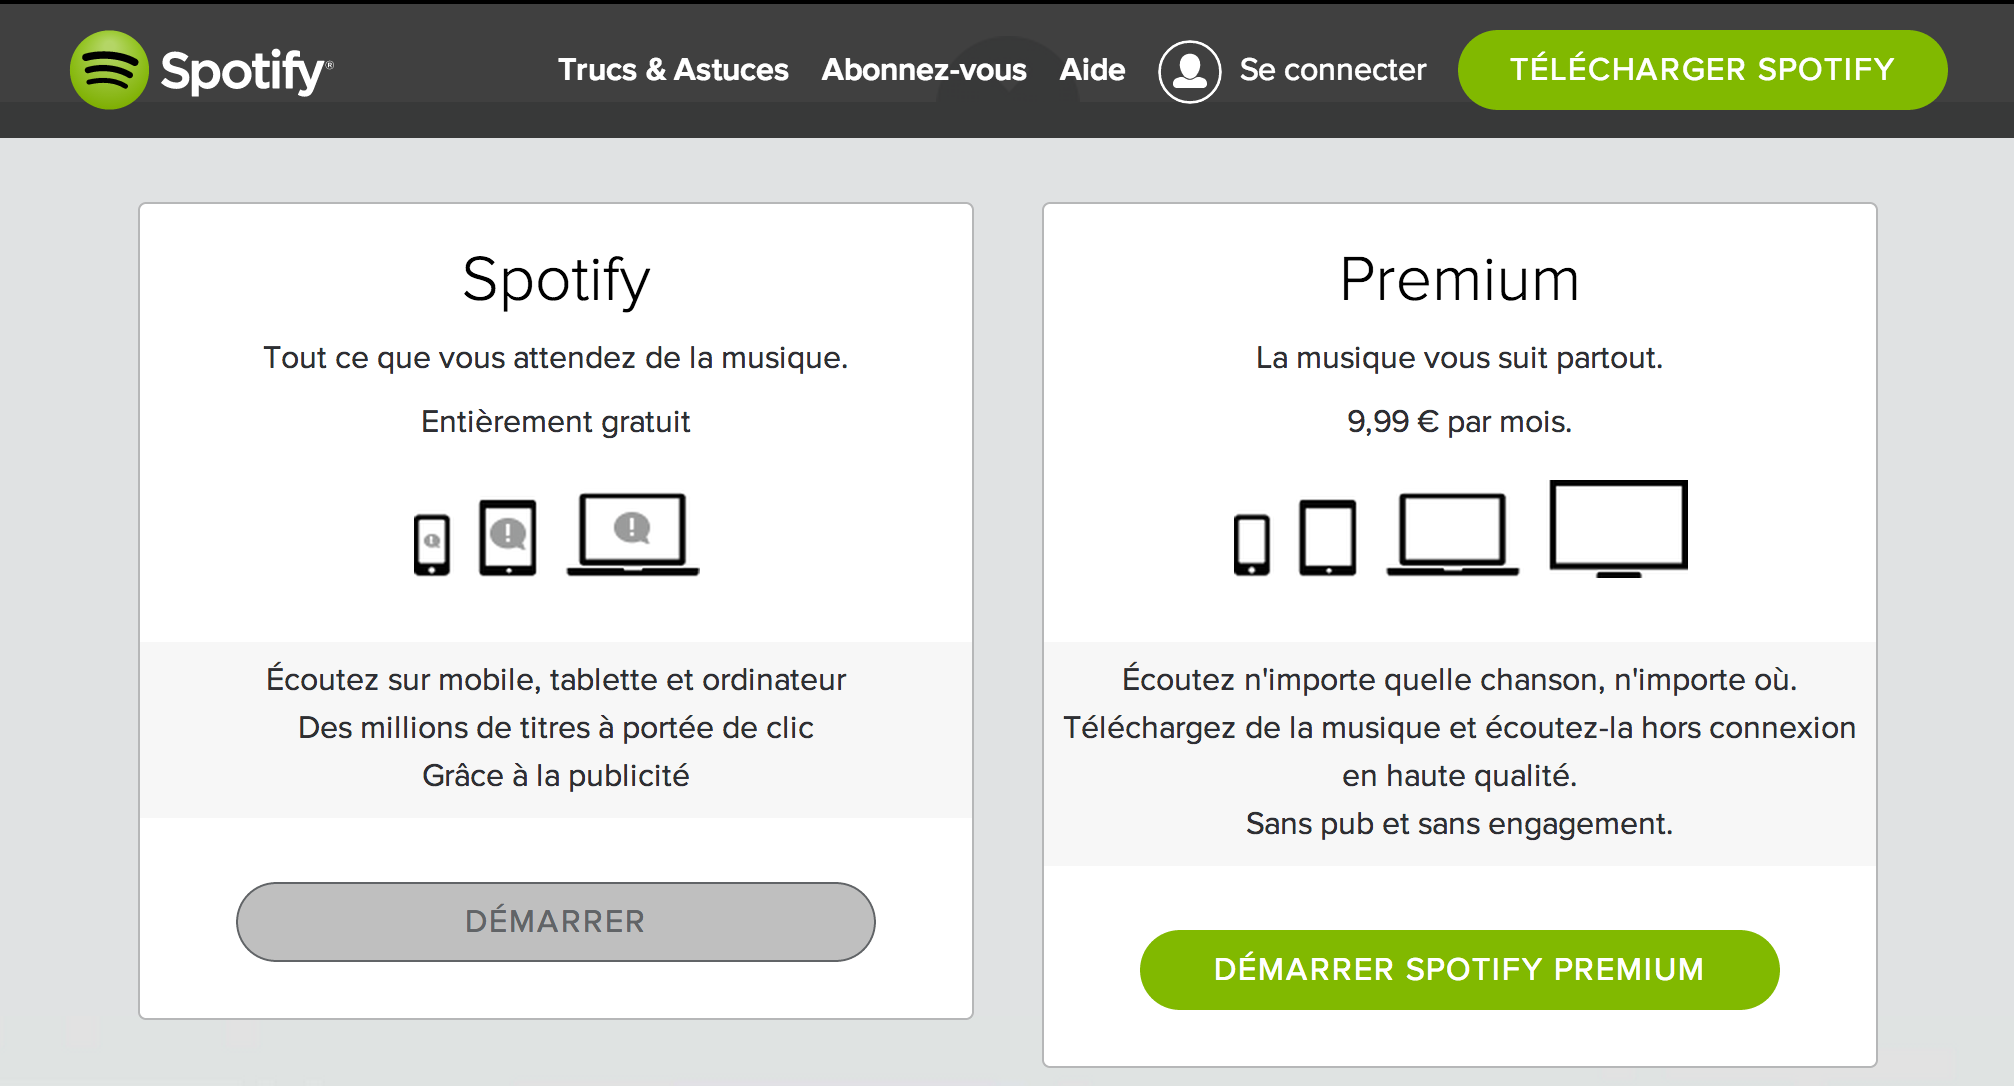
\includegraphics[width=\textwidth]{images/media/premiumSpotify.png}
\end{center}

\paragraph{} %validité et limite du modèle
% citation freemium.org => équations
	\subparagraph{} % comment est-il possible de faire payer 5% de ses clients?
Le concept de freemium peut sembler frauduleux à première vue. En effet, un modèle économique basé sur la distribution gratuite de son produit semble d’emblée voué à l'échec. Il est difficile d'imaginer un boulanger offrant gratuitement ses croissants en espérant financer son affaire via la vente d'offre surclassée comme un croissant avec de la confiture, un sac de transport en tissu issu du commerce équitable et un sourire de la caissière. Une telle pratique économique ne peut être pérenne. De manière générale, toute offre impliquant la disparition du bien\footnote{Les fameux croissants ou tout autre bien de consommation.} ou du service\footnote{Coiffeur, avocat, médecin, ...} après utilisation ne semble pas adaptée au modèle freemium.

\subparagraph{}
Ce qui rend cette solution viable dans le cadre d'un produit digital est le faible coût de duplication et de distribution du produit\footnote{Que ce soit un bien ou un service.}. Un logiciel traditionnel, une fois développé, ne coûte pas plus cher si il est exécuté une fois ou 10 fois sur le poste d'un client. Il en va de même pour les biens culturels\footnote{Le groupe de musique \emph{Nine Inch Nails} a offert son album en mp3 téléchargeable gratuitement. Les supports physiques en édition de collection vendus plus cher qu'un disque conventionnel, les produits dérivés et la vente de billets de concert constituent l'offre premium du groupe. Le coût de distribution et la duplication de fichiers musicaux étant nuls en apparence, l'offre premium paiera les musiciens et rentabilisera les coûts de production sans pour autant engraisser un intermédiaire malveillant.}, un livre une fois écrit et converti dans un format numérique a le même coût de production peu importe le nombre de ses lecteurs. La magie de ce paradigme vient du fait que copier un fichier est une opération logiciel simple qui n’altère ni ne supprime le fichier original quel qu’en soit le nombre de copie effectuée. Le coût de production d'une copie du produit s'approche alors de zéro.

\subparagraph{}
Il ne faut surtout pas considérer un utilisateur gratuit comme une perte car un consommateur ne payant pas le produit n'est pas un client, c'est un moyen. Au même titre que l'achat d’encarts publicitaires, de mots-clef dans les moteurs de recherche ou de publication mise en avant sur les réseaux sociaux pour faire la promotion du produit, un utilisateur est un vecteur de communication virale.



En proposant un service ayant, aux yeux de l'utilisateur, une réelle valeur ajoutée qui le pousserait à l'utiliser régulièrement, on crée une \emph{relation d'approbation} qui a une valeur bien supérieure à la publicité.
En effet, si demain la boucherie de mon quartier adopte le modèle freemium, elle offrirait gratuitement ses produits à tous les clients potentiels et ferait payer un service de charcuterie premium qui serait optionnel.
Il est alors plus que probable que je diffuse l'information auprès de mon réseau qui le diffusera lui aussi à son réseau et ainsi de suite jusqu'à atteindre la limite du marché. Dans ce cas précis, le coût de déplacement serait bien supérieur au gain apporté par le produit gratuit.
Dépenser \$200 d'essence pour obtenir un produit gratuit d'une valeur de quelque dizaines de dollars n'est pas judicieux. Il est toujours envisageable de compter sur une clientèle stupide mais mon expérience du jeu de go m'a appris qu'établir une stratégie basée sur les erreurs potentielles de son adversaire n'est que rarement voir jamais payant.
Considérer ses futurs clients\footnote{aka utilisateurs gratuits ou leur réseau} comme des moutons à tondre ne peut être une stratégie payante à long terme même si à court terme de telles méthodes peuvent apporter des recettes.
\subparagraph{}
Il faut néanmoins se montrer vigilant, les pratiques trop agressives auprès de l'utilisateur l’entraînera peut être à court terme à acheter et augmenter les revenus de la compagnie mais, très vite, l'utilisateur ce lassera et quittera la plate-forme réduisant à néant toute stratégie de rétention d'utilisateurs à long terme. Depuis sa capitalisation boursière la compagnie Zynga\footnote{Zynga, société créatrice de Farmville ainsi que 67 autres jeux gratuits sur le réseau social Facebook, a fait son offre publique initiale, IPO, le 26 décembre 2011 évaluant l'entreprise après son entrée en bourse à environ 7 milliards de dollars.\cite{ipoZynga}} tente d'achever sa profitabilité et adopte une stratégie de plus en plus agressive auprès de sa communauté de joueurs pour augmenter leur consommation et les revenus de la société. Ces campagnes ont eu pour effet une chute drastique, -68.55\% entre le quatrième trimestre 2012 et le troisième trimestre 2014 du nombre d'utilisateurs.
% source http://www.appmtr.com/facebook/app/321574327904696-farmville-2/

\begin{center}
	\begin{tabular}{|l*{1}|c|c|}
		Trimestre  & utilisateur actif mensuel & Variation\\
		\hline
		2012 T4 & 51,569,209 & 0 \\
		2013 T1 & 40,557,507 & - 21.35\% \\
		2013 T2 & 34,713,652 & - 14.41\% \\
		2013 T3 & 26,268,910 & - 24,32\% \\
		2013 T4 & 23,630,665 & - 10.04\% \\
		2014 T1 & 19,339,065 & - 18.16\% \\
		2014 T2 & 22,471,919 & + 16.20\% \\
		2014 T3 & 19,826,868 & - 11.77\% \\
	\end{tabular}\cite{appmtrFarmVille2}
	\label{Evolution du nombre d'utilisateurs mensuels du jeu Farmville 2}
\end{center}

% Les restrictions sur les fonctionnalités (e.g. une version "lite" d’un logiciel) ;
% Les restrictions sur la quantité (e.g. un pack spécifique d’hébergement qui limite à 10 le nombre de base de données que l’on peut créer) ;
% Les restrictions sur le nombre de copie (e.g. un logiciel qui ne peut être installé que sur un unique ordinateur et non sur un réseau) ;
% Les restrictions sur les classes d’utilisateurs (e.g. un logiciel gratuit tant que l’utilisation est non commerciale) ;
% Les restrictions sur l’effort (e.g. un logiciel gratuit mais limité qui peut être débloqué gratuitement mais au prix de démarches laborieuses, qui peuvent être facilitées moyennant un paiement).
\subparagraph{}
Un modèle freemium, si il veut survivre à long terme, doit être conçu et mis en place de manière éthique\cite{ethicalF2P} en respectant les utilisateurs. Beaucoup d'offres freemium cherchent à tirer un maximum de bénéfices, le plus rapidement possible, ce qui semble être en ce moment un plan d'affaire extrêmement lucratif, ne cherchant pas la rétention à long terme des utilisateurs. Dans le cas des jeux gratuits contenant de la consommation dans le jeu, beaucoup fonctionnent exactement de la même manière. Parfois, il suffit de changer l'emballage pour donner l'impression de nouveauté suffisante à délier la bourse des plus impulsifs.

\subparagraph{}
Il est donc fondamental de connaître exactement ses coûts de production et de distribution avant d'envisager un modèle tel que celui-ci. Pour cela, il faut savoir qu'il existe plusieurs types de coût.
Les premiers sont les \emph{coûts fixes\index{Coûts fixes!définition}}\footnote{Exemple de coût fixe: loyer, salaire des employées permanents, frais de justice, etc}\cite{defCoutFixeEtVar}, ils ne varient pas en fonction du volume d'activité de l'entreprise.
À l'inverse, les \emph{coûts variables\index{Coûts variables!définition}\footnote{Exemple de coût variable: consommation éléctrique dans une manufacture, salaire des employés temporaires, location d'instances sur Amazon Web Services pour répondre à la demande utilisateur.}\cite{defCoutFixeEtVar}}\ sont proportionnellement liés au volume d'activité de l'entreprise. Plus cette dernière génère de l'activité, plus ses coûts variables vont augmenter.
Vient ensuite le tour des coûts d'opportunité\index{Coûts d'opportunité!définition}\footnote{Exemple de coût d'opportunité: dépot de garantie à la création d'un compte en banque }\cite{defCoutOpp} qui sont un manque à gagner sur l'exploitation du capital, c'est à dire que dans une situation donnée une somme d'argent à été bloquée ou investie. Si ces actifs n'avaient pas été bloqués, ils seraient utilisés pour l'essort de l'entreprise. Un coût d'opportunité est donc la différence du résultat de l'action effectuée minorée par le gain potentiel d'une autre utilisation de la ressource. C'est donc un coût purement spéculatif.
Finalement, les \emph{coûts marginaux\footnote{Exemple de coûts marginaux: frais d'importation, }}\index{Coûts marginaux!définition}, définissent les frais nécessaires à la production d'une commande suplémentaire. Il cherche à définir la rentabilité prévisionnelle d'une action donnée. Il est lui aussi purement spéculatif car c'est avant tout un indicateur stratégique.
\subparagraph{}
Les coûts doivent être estimés de manière précise afin de pouvoir calculer ce que coûte un utilisateur gratuit. Une fois le coût réel d'un utilisateur gratuit déterminé, il est nécessaire de connaitre le taux de conversion de ses utilisateurs gratuit en utilisateurs payants. Si l'on multiplie ensuite le nombre d'utilisateurs par le taux de conversion qui multiplie la contribution unitaire de chaque utilisateur, on obtient une estimation de ses revenues\cite{équationFreemium}.

%%%% synthèse par les équation %%%%%
\begin{equation}\index{U!définition}
	U\ =\ Nombre\ d'utilisateur\ gratuit
\end{equation}


\begin{equation}\index{T!définition}
	T\ =\ Taux\ de\ conversion
\end{equation}


\begin{equation} \index{Cu!définition}
	Cu\ =\ Contribution\ unitaire\ moyenne\ par\ utilisateur payant
\end{equation}


\begin{equation}\index{Revenue!définition}
	U \times T \times Cu\ =\ Revenue
\end{equation}

Lorsque cet indicateur est calculé, il faut en calculer un second: les coûts variables. C'est à dire une estimation du coût total des utilisateurs gratuits. Pour cela rien de plus simple: multiplier le nombre de vos utilisateurs gratuits par le coût d'un utilisateur. Ces utilisateurs ne sont pas des coûts fixes car le montant exact de leur utilisation dépendra du contexte de l'offre freemium.

%%%%%% synthese equations %%%%%%%
\begin{equation}\index{Cg!définition}
	Cg\ =\ coût\ d'un\ utilisateur\ gratuit
\end{equation}


\begin{equation}\index{Couts variables!calcule}
	U\ \times\ Cg\ =\ Coûts\ variables
\end{equation}

Si en soustrayant aux revenus, les coûts variables et que le résultat de l'opération est supérieur aux coûts engendrés par la création et la distribution du produit alors, théoriquement, le modèle est économiquement viable.

%%%%% synthese equation %%%%%%
\begin{equation}
	C\ =\ Coûts\ fixes\ +\ Couts\ Variables\ +\ Couts\ spéculatifs
\end{equation}
\begin{equation}
	(Revenue\ -\ Couts\ variables)\ <\ C
\end{equation}

% présentation du modéle freemium happybox
\paragraph{} % Happybox avec chiffres
Le choix du freemium pour HappyBox CMS est le résultat de longues discussions avec la totalité de l'équipe lors de l'été 2013. De ces réunions, nous avons établi pour chaque fonctionnalité du produit les limites de l'offre gratuite et nous avons pensé à une solution de monétisation de l'offre premium\footnote{Voir en annexe le document récapitulatif rédigé en Août 2013 par François Lacroix-Durant}.
Trois offres ont alors vu le jour au sein de l'application:

\begin{flushleft}
	\begin{tabular}{|l|l|l|l|}
		Métrique & Personnel & Professionel & Agence \\
		\hline
		Domaine & sous domaine de happyboxcms.me & domaine personnalisé & domaine personnalisé \\
		Nombre de projet & 1 & 25 & illimité \\
		Bande passante & 5GB par mois & 50GB par mois & 100GB par mois \\
		Espace disque & 1 GB & 10 GB & 100 GB \\
		Style & basique & basique & avancé \\
		Analyse de trafic & basique & avancé & avancé \\
		Contenu Dynamique & non compris & non compris & oui \\
		Support & communautaire & via ticket & via ticket et téléphone  \\
		Prix & gratuit & \$49.99/mois & \$100/mois\footnote{Ou négocié en fonction des services demandés.} \\

	\end{tabular}
\end{flushleft}
\subparagraph{}
Il faut, ensuite, appliquer les équations vues dans les paragraphes précédents avec des chiffres prévisionnels basés sur une \emph{croissance\index{startup!croissance} de la masse des utilisateurs de 4\%\footnote{Croissance minimum hebdomadaire d'une startup afin d'attirer des capitaux issus du \emph{venture capitalisme}} selon Paul Graham fondateur de Y-Combinators. 
C'est aussi le taux de croissance prévisionnel défini dans le plan d'affaire de DOM Element Inc..} par semaine.
Spéculons sur un lancement discret en janvier 2014 avec cinquante utilisateurs gratuits triés sur le volet et un taux de conversion faible de 2\%, au vu du coût minimum par contribution unitaire actuelle de \$49.99. Ces chiffres sont volontairement faibles afin de voir si même avec des indicateurs ne permettant que difficilement d'atteindre les objectifs de rentabilité, cela est encore possible. La profitabilité n'étant pas nécessairement un objectif pour une startup, nous verrons pourquoi dans la section sur les modes de financement des startups.


%%% PRESENTATION
\begin{center}
	\begin{tabular}{|l||c|c|c|}
		Temps & Utilisateurs gratuits & Utilisateurs payants & Coût utilisateur\footnote{La méthodologie exacte de calcul du coût par utilisateur est présentée en détail dans la section .}\\ %%%% AJOUTER LE NUMERO DE SECTION
		\hline
		Janvier 2014 & 50 & 1 & \$0.52 \\
		Juin 2014 & 95 & 1.9 & \$0.48 \\
		Janvier 2015 & 291 & 5.82 & \$0.45 \\
		Juin 2015 & 649 & 12.98 & \$0.45 \\
		Janvier 2016 & 1,994 & 39.88 & \$0.44 \\
		Juin 2016 & 4,442 & 88.84 & \$0.44 \\
	\end{tabular}
\end{center}



\subparagraph{}
Il est possible de continuer d'appliquer les formules présentées dans la partie précédente afin de dégager une prévision théorique de revenu. Si le taux de croissance des utilisateurs reste stable durant les trois prochaines années, en Juin 2016 HappyBox CMS devrait compter 4 442 utilisateurs dont 88.84 payant avec un achat unitaire de \$49.99. On obtient, alors, un revenu de \$4,441.8 auquel il faut retrancher les coûts variables de \$1958.77 afin d'obtenir un résultat d'exploitation de positif de \$2483.03.

%%% PRESENTATION
\begin{center}
	\begin{tabular}{| 1*{l} || c | c | c |}
		Temps & Coût variable & Revenu & Résultat hors frais fixes\\
		\hline
		Janvier 2014 & \$26.26 & \$49.99 & + \$23.73\\
		Juin 2014 & \$46.06 & \$94.90 & + \$48.84\\
		Janvier 2015 & \$132.30 & \$291.35 & + \$159.05\\
		Juin 2015 & \$289.82 & \$649.22 & + \$359.4\\
		Janvier 2016 & \$881.63 & \$1,993.18 & + \$1111.55\\
		Juin 2016 & \$1958.77 & \$4,441.8 & + \$2483.03\\
	\end{tabular}
\end{center}


\subparagraph{}
Afin de clarifier ces projections, voilà un graphique synthétisant les projections d'HappyBox CMS en terme de croissance d'utilisateurs et de flux financiers (de ces derniers sont exclus les investissements, les coûts fixes, les coûts d'opportunité, ainsi que les coûts additionnels). Pour plus de statistiques, rendez-vous dans les annexes pour une foule de projections. Il est, bien sûr, évident qu'avec des indicateurs de base\footnote{Taux de croissance utilisateur, taux de conversion, contribution moyenne par utilisateurs payants} plus optimistes les résultats de ces projections seraient meilleurs.

\begin{center}
	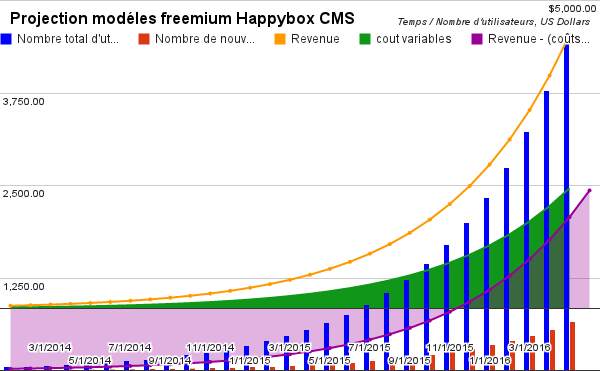
\includegraphics[width=\textwidth]{images/media/chartFreemiumHbCMS.png}
\end{center}


% \paragraph{}%limites

% Un certain nombres de limites sont déjà apparues tout au long de la présentation du modéle.

% - startup pas necessairement en quéte de revenue
% - croissance utilisateur = crédibilité face au investisseur = plus de roulement
% - clientele payante = bon point investissuer ça peu aller trés vite : Jeff Grammer partner Rho Canada startup breakfast montreal
% - source de financement des startup
% - croissance == danger pour les grosse entreprise en place qui ne veulent ==> rachat == objectif atteint
% - Modele freemium interessant pour startup evernote, skype, farmville
% - la croissance est ce qui permet à une startup d'atteindre sa maturité
% - User aquiring = absolue nécessité
% parrallel happybox

% = offre service ou produit gratuit
% - produit de qualité il faut des utilisateurs gratuit et le plus possible.
% - offre premium ajoutant des fonctionnalité payante
% - possible grace au coup quasi nulle de la duplication de bien digitale
% - mais pas que informatique, ex: musique distribution de mp3 gratuit offre premium: fichier de meilleur qualité, vente de support physique edition de collection, billet de concert, ...., nine inch nails album

% - On value un utilisateurs gratuit, c'est une source viral de communication, truc trop cool gratuit == truc géniale donc on en cause au pote qui en cause au pote. Effet de buzz rapide ==> plus d'utilisateur + de potentiel payeur
% - Il faut reellement fournir un service géniale dont les utilisateurs ont besoin! Sinon pas d'utilisateurs

% - taaux de conversion: utilisateur gratuit devenant utilisateur payant
% - Attention il est necessaire de connaitre exactement la valeur d'un utilisateur gratuit.

% - semble insensé mais




		\section{Un produit dans la jungle} % 10 pages
%%%%%%% Intro mise en context %%%%%%%%%%%%%%%%%%%%%
%Putain d'mise en contexte de mon cul!

%%%%%%%%%%%%%%%%%%%%%%%%%%%%%%%%%%%%%%%%%%%%%%%%%%%
			\subsection{HappyBox CMS, une solution complète pour le web.}
		% présentation du produit avec screen et schéma technique (à traduire)

	% abstract
\paragraph{}
HappyBox CMS est un logiciel en tant que service\index{SaaS!HappyBox CMS}, c'est à dire qu'aucune installation n'est requise pour pouvoir l'utiliser. Il fonctionne sur un modèle client-serveur où le client est une page web dans votre navigateur communiquant avec un Service web, le serveur. Il faut le voir comme une feuille d'acétate qui se dépose sur un nom de domaine existant et permet instantanément de créer un site web ou d'en éditer le contenu.

% Dom Element Inc c'est une stratup donc orienter sur 1 seul et unique produit
%\subsubsection{Front end}
	% Présentation utilisateurs
	\paragraph{}
HappyBox est avant toute chose un système de gestion de contenu\footnote{appelé aussi CMS, Content Management System}. Il s'agit d'un logiciel permettant la création et la mise à jour dynamique de site web.
C'est un CMS spécialisé dans la création de site web à une seule et unique page, appelée aussi \emph{page d’atterrissage} ou \emph{landing page} en anglais. Ce type de site web est généralement réservé au opération de promotions, qu'elles soient personnelles\footnote{Page personnelle, présentation d'un projet, CV en ligne, loufoquerie, ...} ou corporatives\footnote{Bon de réduction, présentation d'un produit, événements, ...}. Il a pour objectif d'intéresser les internautes afin de les informer ou de les guider vers un autre service.

%%%%%% TODO: causer SEO %%%%%%

%%%%%%%%%%%%%%%%%%%%%%%%%%%%%%

\paragraph{}
L’accès au service ce fait via une page HappyBox présentant les différentes fonctionnalités du logiciel. Cette page offre aussi un accès aux différents portails communautaires et à la création de compte. Ce site est une vitrine des possibilités offertes par le CMS. C'est le point d'accroche de la communication autour du produit.

%% SCREENSHOT ACCEUIL HAPPYBOX %%

\begin{center}
		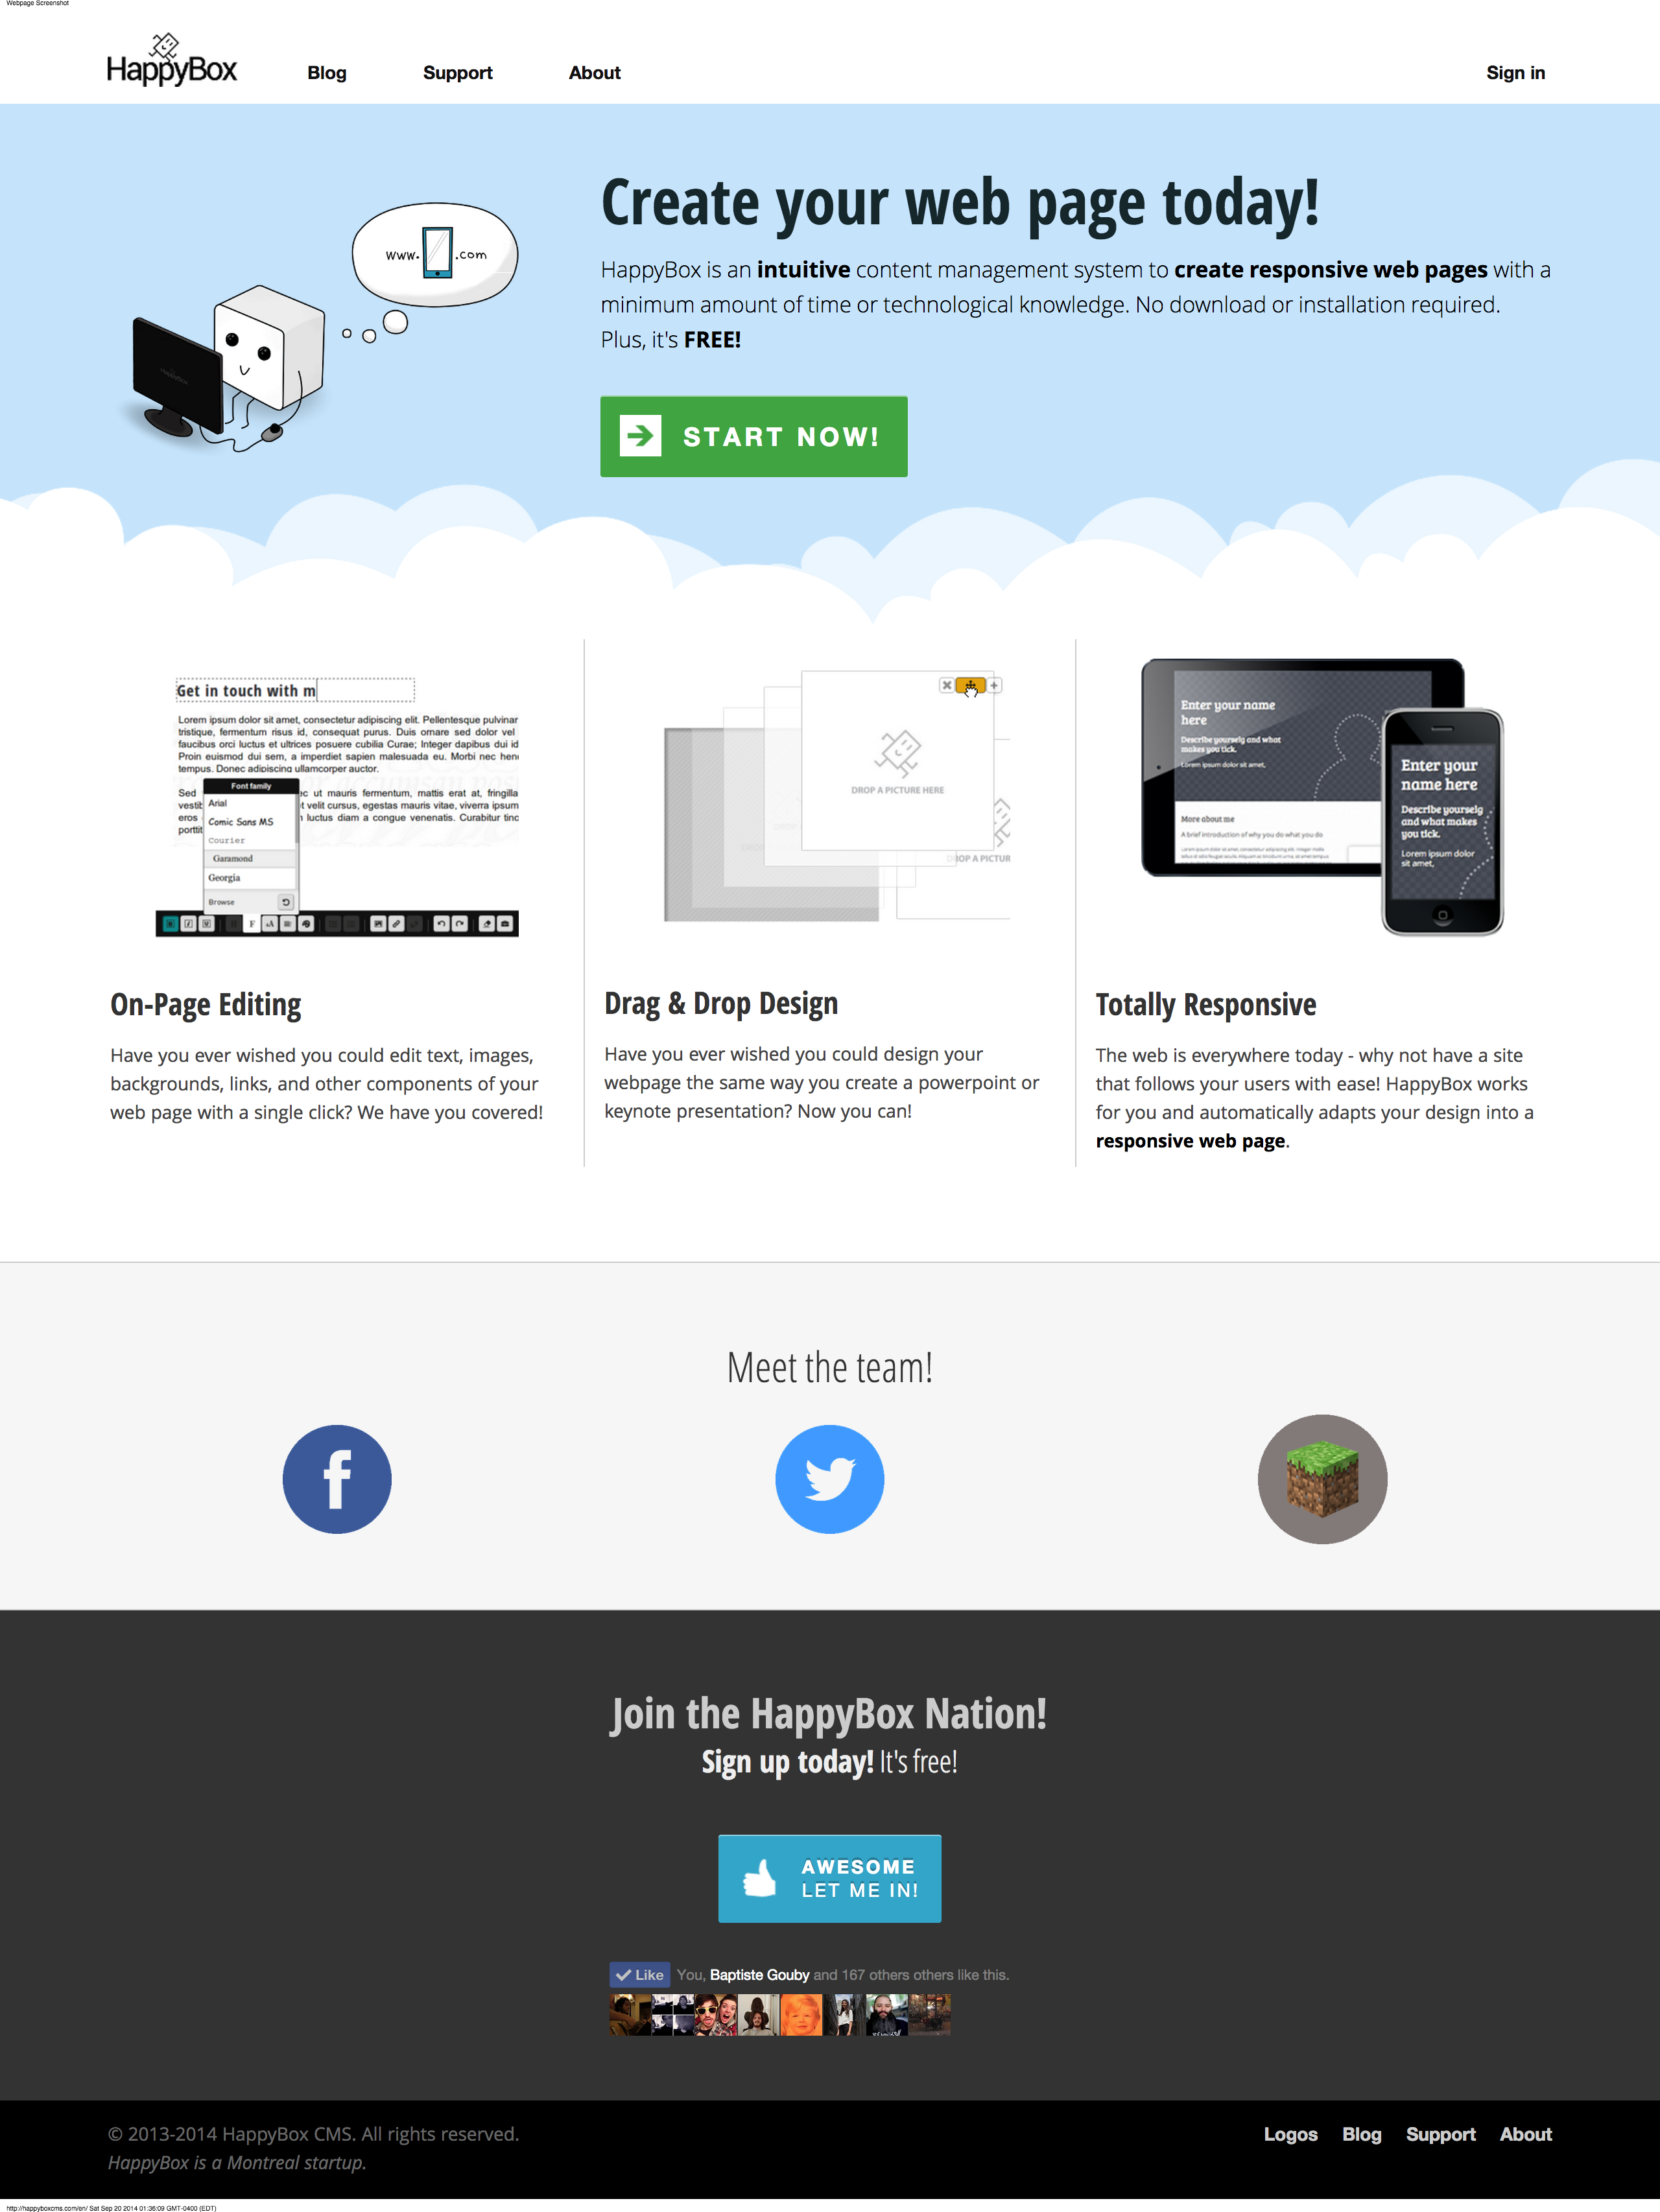
\includegraphics[width=\textwidth]{images/HBscreen/fullLanding.png}
		\caption{\url{http://happyboxcms.com} - Page d'aterrissage}
\end{center}

\paragraph{}
HappyBox CMS propose un éditeur de page intuitif, permettant en quelques clics de définir un gabarit ou template de page. Le moteur se base sur un système de grille. En effet, les pages sont définies comme étant un ensemble de lignes ou sections superposées les unes aux autres. Ces lignes peuvent être visibles ou non afin de créer des séparateurs sur la page\footnote{Section invisible laissant apparaître le fond de la page.}. Dans ces sections, il est possible de définir des colonnes d'une largeur définie lors de la création du gabarit. Ces colonnes sont des conteneurs qui nous permettrons de stocker le contenu de la page par l'intermédiaire de \emph{widget\footnote{Élément textuel, titre, images, formulaire de contact, liens, ...}}.

Chaque gabarit est complètement \emph{responsive\index{responsive!moteur de gabarit}}, c'est à dire qu'il s'adapte automatiquement à la résolution du navigateur client afin de garantir la meilleure expérience d'utilisation, quelque que soit la plate-forme utilisée pour consulter un site créé avec HappyBox CMS. La fonction de prévisualisation ainsi que les boutons en bas de l'éditeur permettent de tester son site pour chaque type d'appareil.


%% SCREENSHOT EDITEUR DE GABARIT%%
\begin{center}

		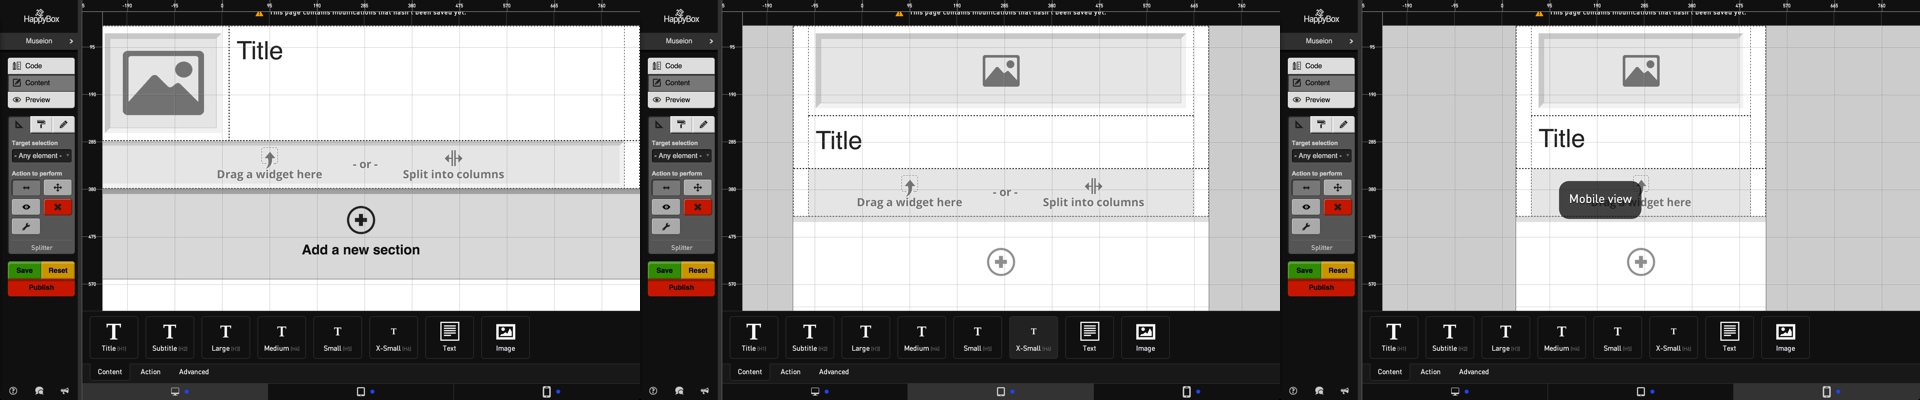
\includegraphics[width=\textwidth]{images/HBscreen/editeurGabarit.png}
		\caption{Editeur de Gabarit: vue ordinateur, vue tablette, vue mobile}

\end{center}

\paragraph{} % contenu, style, SEO
Une fois qu'une page est structurée, il faut lui ajouter un style. Pour cela, un éditeur de style complet permettant de gérer la majorité des propriétés css via une interface simple d'utilisation permet aux non-développeurs d'affiner leur design avec un niveau de détails inégalé. Pour les utilisateurs confortables avec l'édition d'un fichier css, il est possible d'écrire directement du code css dans l'éditeur.
Le contenu de la page (textes, images) est éditable directement sur la page avec un rendu en temps réel. Ce que vous voyez c'est ce qui sera affiché.
HappyBox a été pensé en gardant en mémoire qu'une page d’atterrissage est avant tout un outil de référencement permettant d’offrir une meilleure visibilité à un produit ou un service dans le web. C'est pourquoi, un assistant de SEO est disponible dans l'éditeur. Il propose d'améliorer votre page en temps réel afin que les moteurs de recherche indexent au mieux la page.
%% screen contenue style CEO
\begin{center}
	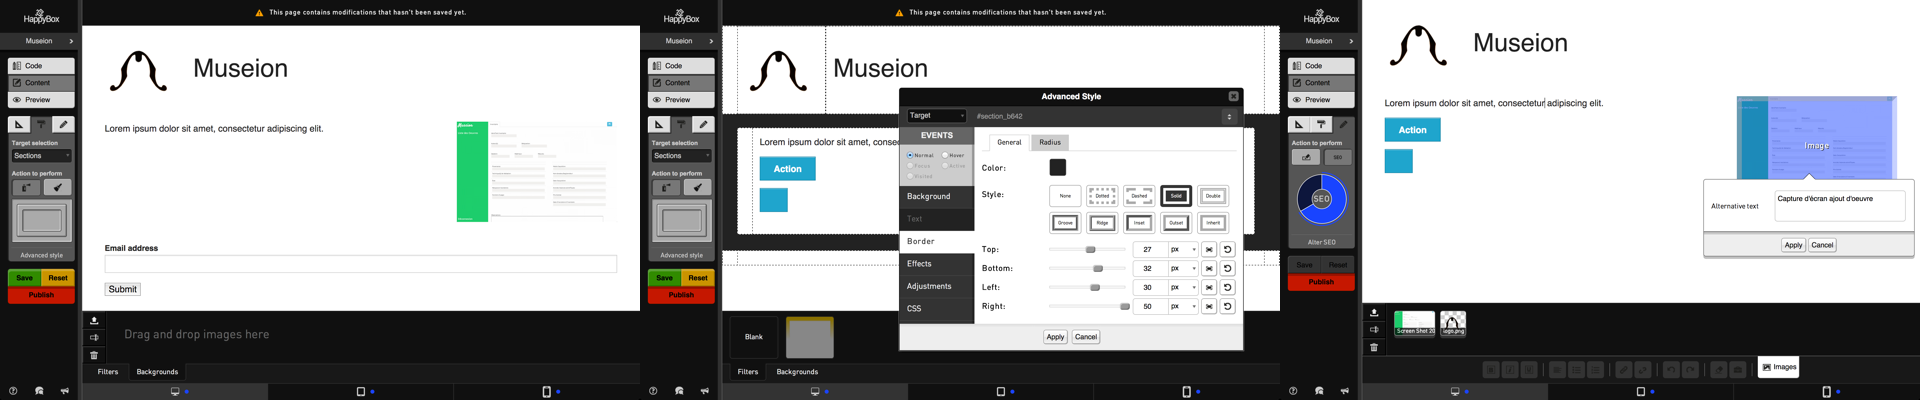
\includegraphics[width=\textwidth]{images/HBscreen/contenueStyleSeo.png}
	\caption{Editeur de contenue, editeur de style, editeur de SEO}
\end{center}

\paragraph{} % editeur de code + versionning
HappyBox cible prioritairement les développeurs web. C'est pourquoi, il est doté d'un éditeur de code permettant d'éditer l'intégralité des sources de la page et d'ajouter des modules php ou javascript afin d'étendre encore les possibilités de la plate-forme. Ce qui n'est pas déjà développé par l'équipe, pourra être développé et tester par l'utilisateur. Le tout avec un rendu en temps réel.
%% Screenshot editeur de source
\begin{center}
	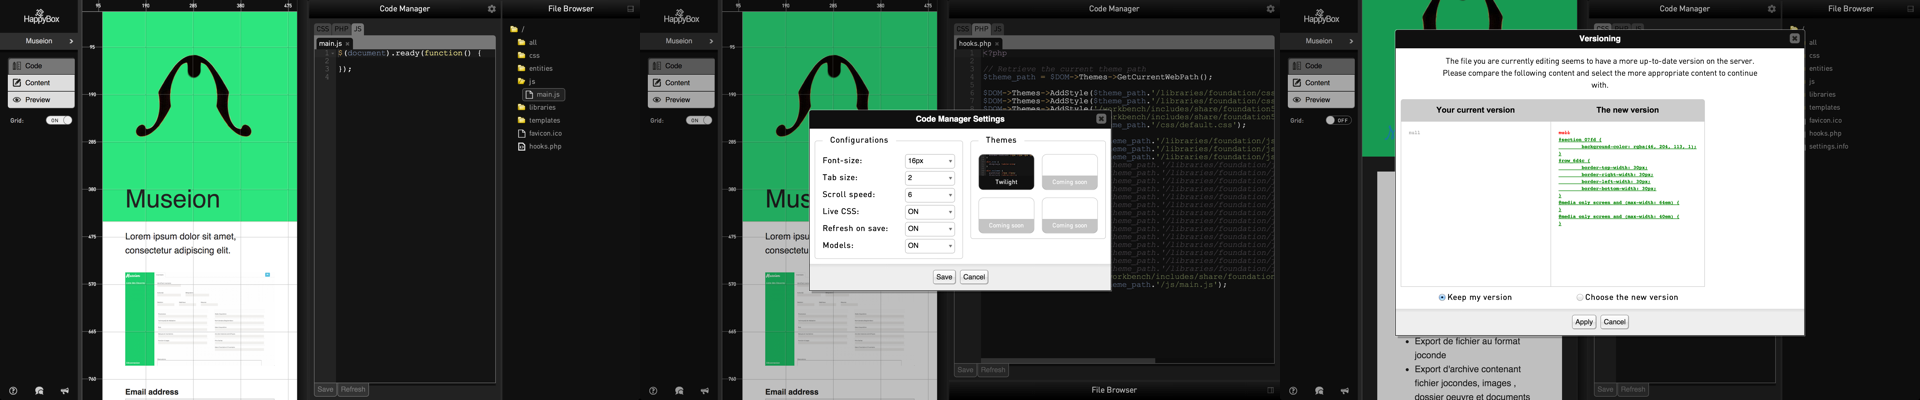
\includegraphics[width=\textwidth]{images/HBscreen/codeManager.png}
	\caption{Editeur de code: fichier php, configuration, gestion des versions}
\end{center}

% séparation fond et formes
\paragraph{}

Toutes ces fonctionnalités ont pour finalité la création d'une page web unique. Il est donc possible de la prévisualiser comme les utilisateurs la verraient et ce sur chaque type de résolution.
\begin{center}
	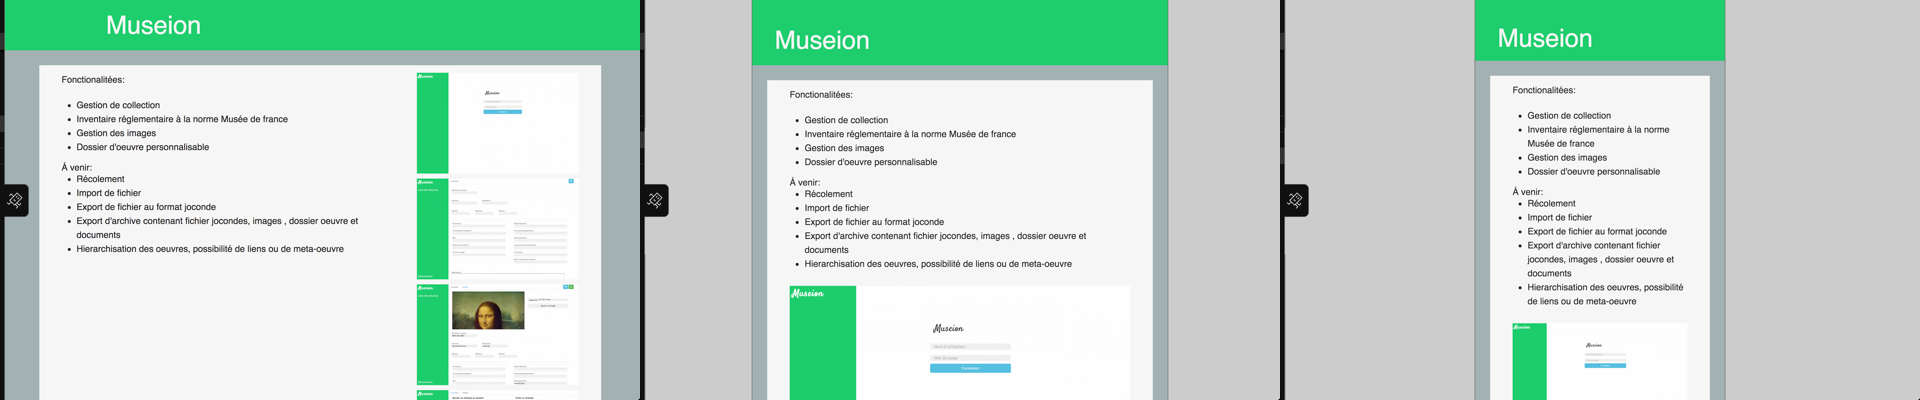
\includegraphics[width=\textwidth]{images/HBscreen/preview.png}
	\caption{Prévisualisation de la pages version ordinateur, tablette et mobile}
\end{center}

% présentation des outils de gestions
\paragraph{}
De plus chaque client se voit alloué un espace dédié sur nos serveurs. Il reste ainsi le seul et l'unique propriétaire de ses données. HappyBox est donc aussi un hébergeur de données. Afin de répondre à cette seconde problématique, un ensemble d'outils est mis à la disposition de l'utilisateur. Ces derniers servent à accéder à ses statistiques d'utilisation de stockage, la gestion des noms de domaines ainsi que l'analyse du trafic sur ses pages.

\begin{center}
	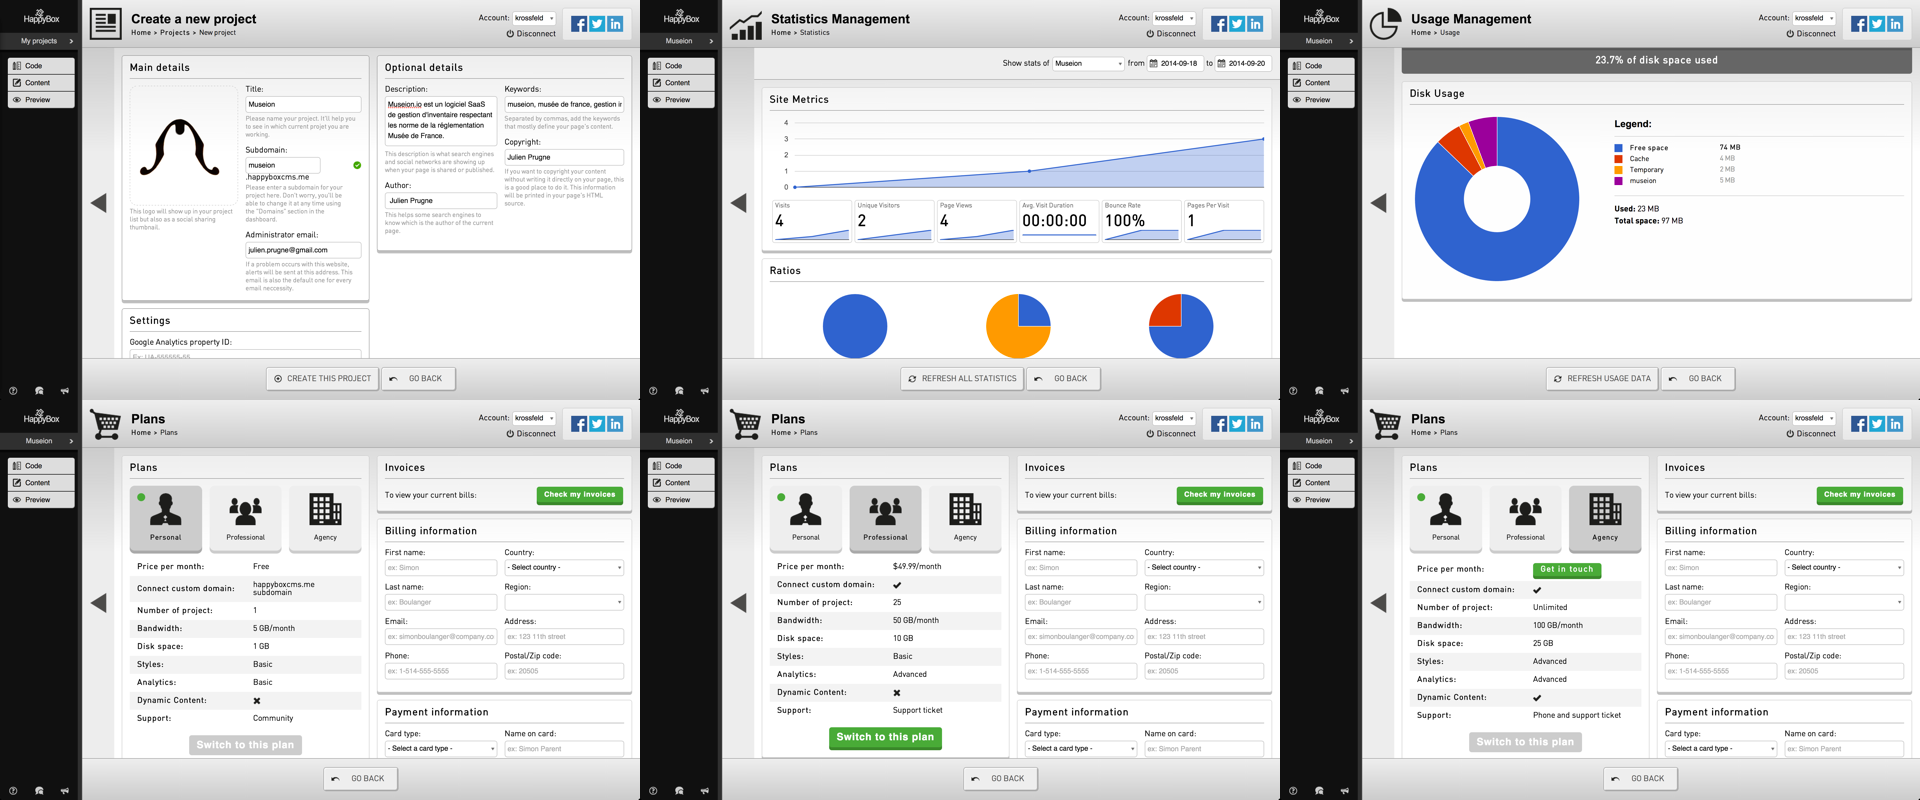
\includegraphics[width=\textwidth]{images/HBscreen/dash.png}
	\caption{Les différentes options du panneau d'administration et les différents forfaits proposés}
\end{center}


	\subsection{Étude de l'écosystème des startups}

% http://blogs.wsj.com/accelerators/2013/06/24/steve-blank-the-6-types-of-startups-2/
		\paragraph{Présentation de 6 principaux\cite{typeStartup} types de startups}

			\subparagraph{Le style de vie startup:} %style de vie
Le premier type de startupeur cherche un projet et une équipe plus qu'une structure économiquement viable. Il ne travaille pour personne et souhaite vivre de sa passion. Typiquement, il est un surfer californien offrant des leçons de surf pour payer les factures et passer un peu plus de temps sur sa planche. Il ne s'agit pas réellement d'une startup dans le sens où son objectif n'est pas de \emph{démarrer} et de connaître une croissance rapide.

			\subparagraph{Les petites entreprises:} % petite entreprise
Les seconds sont des entrepreneurs opérant dans des petites entreprises, ils sont généralement boucher, coiffeur, développeur, et bien d'autres choses encore. Ils ont créés leur structure grâce à leurs économies ou l'argent qu'ils ont pu emprunter. Ils ne correspondent pas non plus à l'image médiatique des entrepreneurs et leur compagnie n'est pas adaptable à un marché de masse. Ils ne sont pas pour autant négligeables, en terme de statistique, c'est le profil majoritaire des entrepreneurs.

			\subparagraph{Les mandatés par une plus grosse structure:} % filiale grosses entreprise permettant de tester de nouveaux modèles
De nos jours, la plupart des grosses entreprises se sentent menacées par ces nouveaux acteurs à croissance démentielle. Elles ont donc essayé de trouver une parade afin de garantir un flux continu d'innovation dans les méthodes d'affaire ainsi que dans le développement de nouvelles technologies. Les fondateurs sont mandatés par une entreprise afin d'externaliser un développement et de prendre un minimum de risque pour la filiale mère. Ces grosses entreprises possèdent les fonds nécessaires au développement de sa filiale qui lui garantira une survie et un rachat si les objectifs sont atteints. Cette pratique permet de déroger aux pratiques managériales et à la hiérarchie souvent lourde, il est ainsi possible de développer le produit (bien de consommation, services, brevet(s), ...). Ce sont des laboratoires technologiques limitant les risques\footnote{En cas d’échec seuls les fonds investis sont perdus.}

			\subparagraph{Startups à vocation sociale} % à vocation sociale ex I can go without
Ce type de startup est unique, il ne cherche pas prioritairement à vendre un produit ou un service commercial. Les fondateurs sont des idéalistes ayant un plan pour améliorer le monde ou essayer en tout cas.
Il peut s'agir d'organisme à but non-lucratif, lucratif ou hybride alliant ainsi le meilleur des deux mondes.
En effet, une startup vivant principalement par ses flux entrant de capitaux entrant, il peut être nécessaire d’offrir un modèle intégrant une perspective de rentabilité en plus de sa vocation philanthropique et un placement intéressant en terme d'image pour l'investisseur ou le mécène. Leurs sources de financement sont  multiples: dons, mécénats, venture capitalism, anges des affaires, financement participatif, subvention, ...
C'est un modèle particulièrement adapté à des missions humanitaires, des projets de développement durable.


			\subparagraph{Les \emph{tout doit disparaitre}, créer pour être vendu} % Buyable ex: dev dúne techno puis vente trouver des exemples
Ces structures n'ont qu'un seul objectif: créer un produit pouvant être vendu le plus vite possible et le plus cher possible. Majoritairement, les fondateurs de telles structures sont expérimentées et ont un domaine d'expertise poussé\footnote{Quel qu'en soit le domaine.}. Ce qui leur permet d'analyser le marché et d'y trouver des niches d'innovation. Ces niches doivent être exploitées rapidement afin d'arriver avant que la concurrence ne se soit créée. Elles proposeront ainsi un produit ayant une valeur ajoutée importante car unique ou technologiquement supérieure à ses concurrents. Une fois que ces structures ont vendu leur société pour une somme généralement comprise entre \$500,000 à \$50,000,000, ces startupeurs cherchent une nouvelle pépite d'innovation qu'ils pourront financer avec une partie de la vente de la compagnie précédente.

	%%%%%% IMAGES %%%%%%
			\subparagraph{Les évolutives} %scalable % google, Facebook, doyourfreemi
Finalement, viennent les startups conçues dans leur essence pour l'évolutivité. Ces compagnies visent généralement des taux de croissance extrêmement rapides et nécessitent des fonds importants permettant de soutenir leur besoin de croissance; principalement des fonds d'investissement gérés par des investisseurs appelés \emph{venture capitalism\footnote{Capitalisme d'aventure}}. La majorité de ces startups mourra avant de connaître le destin glorieux et porteur de millions correspondant au mythe de la startup. Ce fut, néanmoins, le cas de Facebook, Google ou encore Twitter qui sont des exemples de startup ayant basée leur stratégie sur l'adaptabilité et l'évolutivité et sont devenues des méga-corporations internationales ne se limitant plus à leur domaine d'origine.

		\paragraph{La chaîne d’approvisionnement }

L'économie traditionnelle peut être définie par sa chaîne de distribution des biens, dans ce modèle un \emph{fournisseur/créateur} vend sa production à une \{plate-forme de centralisation des biens} qui se chargera ensuite de la distribuer et de la vendre au consommateur. Le concept est simple: acheter à moindre coût pour ensuite revendre à un prix supérieur. Ceci permet de dégager une \emph{recette} qui doit être supérieure à la somme du coût d'achat. Si la recette est supérieure aux coûts alors l'opération génère des bénéfices qui peuvent être réutilisés dans l'entreprise créant ainsi un cercle vertueux d'investissement.

D'autres modèles d'approvisionnement proposent d'offrir un service gratuit aux consommateurs tout en achetant les biens qui leur sont distribués.
L'injection de publicité dans le service permettra de monétiser ce dernier. Mais méfiance, car ceci n'est possible que si beaucoup d'utilisateurs utilisent le produit gratuit. En effet, ce n'est pas la publicité en elle même qui représente une valeur ajoutée, mais sa diffusion devant un public aussi important que possible. C'est notamment, la méthode de fonctionnement des journaux gratuits, de certaines chaînes de télévision, YouTube par exemple. La seule réelle condition d'un tel modèle est d'avoir une large base d'utilisateurs permettant de valoriser la diffusion de la publicité.

L'industrie du disque, par exemple, à adopter un modèle bi-directionnel. Ce qui signifie qu'un musicien \emph{doit} payer une maison de disque par l’intermédiaire de commission\emph{Et plus insidieusement, par la perte de ses droits sur son travail car l'artiste ne possède que le droit d'en être l'auteur mais la maison de disque possède les droits sur les enregistrements.} pour qu'elle enregistre, et distribue son travail auprès des consommateurs afin que ces derniers aient l'opportunité de l'acheter. C'est un modèle qui ne favorise que l'acteur central qui touche des recettes à la fois de ses clients et de ses fournisseurs.

La proposition de chaîne d'approvisionnement par les utilisateurs, peut être explorée mais ce modèle compte sur l'autonomie des utilisateurs à s'amuser les uns avec les autres. Les utilisateurs créent et consomment le contenu, le tout gratuitement et pour toujours. C'est à mon goût une vision naïve car il est impossible de maintenir un niveau de qualité permettant d'attirer de nouveaux utilisateurs. De bons exemples du modèle UGC\footnote{User Genrated Content} sur les plate-formes web serait \emph{tumblr}, qui propose un service de blogging communautaire gratuit mais la majorité des plate-formes UGC ressemblent plus au site \emph{4chan} et ce n'est pas particulièrement esthétique.

Tous ces modèles de gestion sont intéressants. Ils apportent chacun leurs avantages et leurs inconvénients, mais ils ne peuvent répondre au besoin de croissance d'une entreprise adoptant le modèle freemium.

Une chaîne de distribution différente s'est alors créée autour de l’écosystème de ces entreprises à forte croissance et au potentiel énorme. Plusieurs niveaux de financement sont accessibles aux entreprises présentant de forte chance de rentabiliser l'investissement rapidement. Les startups ont, certes, un énorme taux d’échec mais en cas de revente, elle représente un taux de retour sur investissement suffisant à compenser les pertes dues aux échecs.

		\paragraph{Aparte sur financement des startups}

Il existe deux grands types de récolte de fond pour une startup: les subventions directes et les subventions indirectes.
Les subventions directes sont obtenues via des bourses, lors de la participation à des concours entrepreneuriaux DOM Element a ainsi récolté entre avril 2013 et février 2014 \$40,000 afin de développer la compagnie. Il ne s'agit pas là de prêt ou d'achat de participation au capital, mais juste des fonds données sans volonté de retour sur investissement. Beaucoup d'entreprises financent le début de leur activité de cette manière à Montréal.

\subparagraph{}
Les subventions indirectes correspondent à des prises de part décisionnelle en échange de financement. Les premiers investisseurs sont des proches ou des membres du réseau privé achetant quelque parts pour une somme modique. Les employés rejoignant la compagnie dans ces premiers temps se voient attribuer des \emph{parts de la sueur} qui, en cas de réussite, transforment les employés en millionnaires instantanés.
Les premiers investissements privés sont généralement des fonds provenant d'anges des affaires. En plus du financement, ce genre d'opération entraîne une relation de mentorat. Les anges des affaires sont des particuliers ayant généralement fait fortune dans les affaires et investissant leurs gains dans de jeune entreprise innovante. Ces transactions représentent généralement une prise de capital à hauteur de 10\% à 20\% contre des sommes allant de \$50,000 à \$1,000,000. Cette ronde de financement est appelée \emph{seed}.

\subparagraph{}
Après ces premiers financements, si les résultats sont au rendez-vous, une startup cherchera de l'investissement de série A, B ou AAA\emph{Réserver aux compagnies ayant fait leurs preuves.}. La différence entre ces trois types porte sur les montants proposés par l'investisseur. Ce qui peut représenter plusieurs centaines de milliers de dollars, voir même plusieurs dizaines de millions de dollars.

\subparagraph{}
La dernière étape est généralement la capitalisation. Car ce système qui consiste à obtenir plusieurs rondes de financement est une pratique qui coûte cher et, surtout, la procédure est extrêmement longue. Elle implique d'engager les services d'une banque d'affaire qui définira la première offre publique de valuation, c'est à dire un nombre défini d'action à un prix fixé à l'avance ainsi qu'un pamphlet de plusieurs pages révélant tous les détails financiers et les projets d'évolution de l'entreprise. Cette offre deviendra publique le jour de son IPO\footnote{Initial Public Offering}. La banque en charge de l'introduction propose ensuite à des groupes d'investissements cette offre. Lorsque la banque a réuni assez de réservations pour l'introduction en bourse, alors et seulement à ce moment là, elle annonce la date d'introduction.  Le jour même, la banque achètera l'intégralité des actions puis les redistribuera à leurs nouveaux propriétaires.
Le processus est très complexe et ne concerne qu'une infime fraction des startups.

\subparagraph{}
L'économie des startups est extrêmement spéculative et elle génère des sommes colossales à partir de peu. Historiquement, les bulles spéculatives ont tendance à exploser lorsque la valeur des actifs en circulation sur le marché est supérieure au nombre d'actifs présents. Cependant, il est important de rappeler qu'en 1929, l'économie mondiale s'est effondrée lorsque le marché réel de l'argent n'a plus été capable de soutenir la croissance due aux spéculations. Ce qui démontre, à forte raison, que l'économie spéculative est un jeu potentiellement très dangereux pour l'économie mondiale bien qu'à l'heure la tendance semble inverse. Cette économie paraît être encore une des rares capable de générer de la croissance dans des pays occidentaux qui ont une croissance quasi nulle.

%%%%% SCHËMA RËCAPITULATIF DU CYCLE DE VIE D"UNE Startup

%%%% FINACEMENT HB %%%%%
%Avril 2013 Fondation Montréal Inc. (12 000)
%Juin 2013 Jeunes Promoteurs (18 000)
%Février 2014 SDEVM (10 000)

\subsection{Secteur à forte concurrence}


\begin{center}
	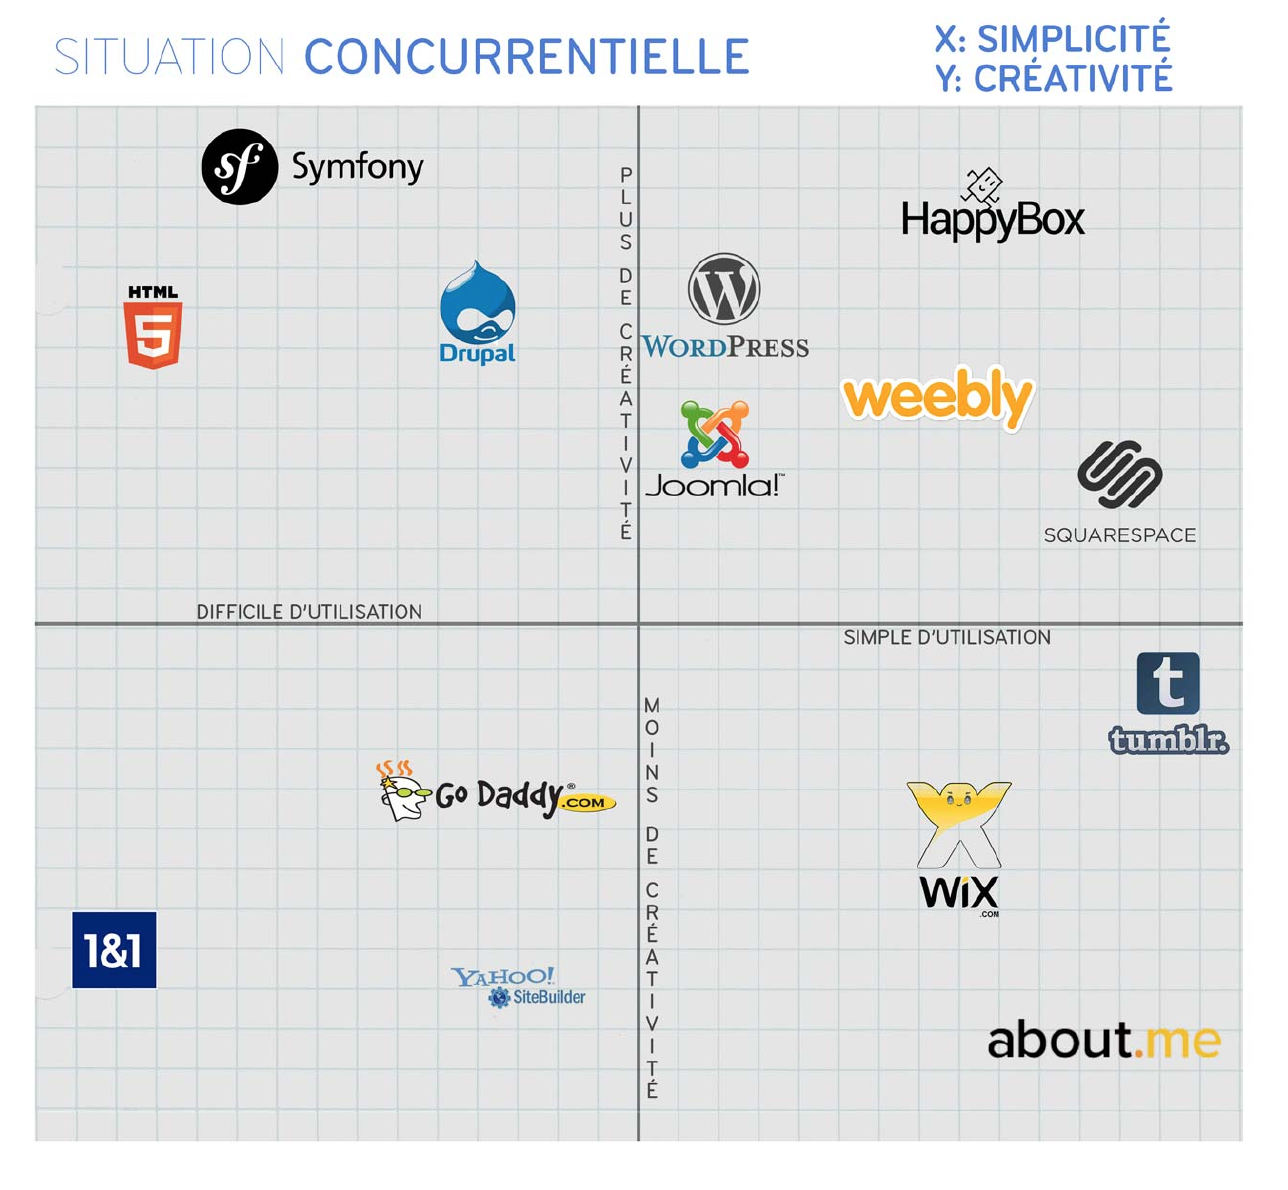
\includegraphics[width=\textwidth]{images/media/concurenceHBCMS}
\end{center}
%%%%%%%%%%%%%%%%%%%%%%%%%

		\paragraph{Critique}
		% VC et angel fournisseur d'un bien précieux du pognon
		% une startup meurt ou multiplie les capitaux
		% explosion bulle spéculative 29, bulle internet, Sub primes
			% actif en circulation ne represente pas la valeur réel =>
		% critique du modéle


	%\chapter{Problématique} % 28 pages
		\section{problématique} % 5 pages

% de gagner en performance, en disponibilités, de simplifier les taches d'administration en faisant abstraction de la couche matérielle.


Dans le cadre d'une startup naissante il est courant de recourir aux services de cloud\footnote{appelé aussi en informatique nuage} public afin de proposer une infrastructure évolutive capable de répondre à une croissance rapide de la base d'utilisateurs et de s'adapter en conséquence.
Mal grès leurs apparences attirantes\footnote{très haute disponibilité, flexibilité, sécurité, faible coût annoncé ...} les plate-formes dites IaaS\footnote{Infrastructure as a Service ou en français : Infrastructure en tant que Service}, engendre un lot de coûts cachés et de nouveaux défis dans la gestion des systèmes d'information.
De plus, l'adoption du modèle freemium impose d'obtenir un nombre critique d'utilisateurs gratuits tout en minimisant au maximum les coûts d'exploitations logiciel afin d'obtenir le plus faible coût par utilisateurs.
Il semble donc nécessaire de mettre en place une politique de gouvernance afin de réellement exploiter le potentiel de telles infrastructures pour achever un taux de croissance important, un coût par utilisateurs minimale et une capacité d'adaptation optimale. Comment et par le biais de quels indicateurs pouvons-nous atteindre cet objectif?


			%Explication et développement de la problématique
			\subsection*{}
				%terminologie
				%\subsubsection*{}

Avant d'aborder le vif du sujet il me semble nécessaire d'expliciter un certain nombre de termes et concepts qui sont utilisés dans la problématique et s'avèrent fondamentaux à la compréhension de ce document.
					%cloud
					%\paragraph{}
						%definition Cloud computing en géneral

Le cloud computing\cite{cloudDef}\index{Cloud computing!Définition} est une pratique visant à dématérialiser les infrastructures des services d'information. Elle entraîne un changement fondamental dans le paradigme d'accès aux ressources informatiques. En effet, les machines hôtes ne sont plus accessibles physiquement mais virtualisées à l'aide d'un hyperviseur\index{Hyperviseurs}.

Les hyperviseurs sont des plate-formes de virtualisation permettant d’exécuter plusieurs systèmes d'exploitation dit invités\index{système invité} sur une même machine dite hôte\index{système hôte} ou une ferme de calcul\footnote{Appelé également grappe de serveurs ou encore cluster. Il s'agit d'un ensemble d'ordinateurs reliés les uns aux autres, mettant leurs ressources en commun, créant ainsi une sorte de \emph{super ordinateur}. }.

Cela crée ainsi une abstraction entre la gestion physique du matériel et l'exploitation des ressources informatiques. Ainsi, la mise en place d'un serveur ne se fera plus en achetant et en installant un nouvel hôte dans son centre de données, mais via la réservation et la création de machines virtuelles.

Un hôte physique hébergera donc un ou plusieurs systèmes d'exploitation et l'hyperviseur se chargera d'allouer ou non les ressources\footnote{unité de calcul, mémoire, stockage, accès réseau, ...}  physiques nécessaires via des interfaces virtuelles accessibles depuis la machine virtuelle comme si ces derniers étaient physiques. Le système invité se comportera comme si il possédait son propre matériel.

Les nuages peuvent être classés dans deux catégories: les cloud privés et les cloud publics.

						% définition cloud privé

Les cloud privés\index{cloud privé|nuage privé! définition} sont des infrastructures physiques\footnote{serveur isolé ou en grappe} louées ou hébergées dans un centre de données et uniquement utilisées par le locataire ou propriétaire. Ces cloud sont physiquement accessibles par les administrateurs qui seront responsables de leur bon fonctionnement. Si les ressources fournies par le nuage privé viennent à manquer, il sera du ressort des exploitants\footnote{propriétaire ou locataire des infrastructures} d'acheter, de configurer et d'installer un nouvel hôte dans la ferme de calcul afin d'augmenter les ressources allouables aux systèmes invités. Á puissance égale ces infrastructures semblent moins dispendieuses que les cloud publics mais les moyens humains nécessaires à la mise en place et la maintenance de telles solutions sont conséquents.

						% définition cloud public
Les seconds, dis nuage public\index{cloud public|nuage public! définition}, sont des infrastructures accessibles généralement via des applications web et/ou des interfaces de programmation\footnote{API: Application Programming Interface}. Les ressources sont accessibles en libre service et à la demande. Le prestataire facturera à l'utilisation\footnote{Exemple: volume de données hébergées, mémoire utilisée par une application, bande passante, ...} ou de manière forfaitaire\footnote{Location annuelle d'une instance, réservation d'un espace de stockage dédié, ...}.

					%\paragraph{IaaS/PaaS/SaaS} transition TODO:definir serrvice web
					%utiliser pizza as a service comme exemple
				% résumé
Les cloud publics sont généralement composés de trois types de services\index{service|service web!définition}\footnote{Un service web\cite{webServicesDef} peut être défini comme étant une interface logicielle permettant un accès standardisé à un ensemble de ressources hétérogènes via internet ou un réseau intranet.}:
\begin{description}

	\item[IaaS\index{IaaS|Infrastructure as a Service}, Infrastructure as a Service, Infrastructure comme un Service] Amazon Web Services, Google Compute Engine, Digital Ocean

	\item[PaaS, Plateform as a Service, Plate-forme comme un Service] Heroku, Google App Engine, dotCloud, Amazon Opswork

	\item[SaaS, Software as a Service, Logiciel comme un Service]
	Happybox CMS, Gmail, Jira, Museion

\end{description}

Pour bien expliquer ces différents concepts, nous nous référerons à l'excellente analogie \emph{Pizza comme un Service}\cite{PizzaasaService}. Cette dernière nous explique que les habitudes d'utilisation de plate-forme en ligne sont comparables aux habitudes de consommation de pizza.

En effet, un cloud privé\index{Cloud privé!Définition par la pizza} où vous vous chargeriez d'équiper les locaux en électricité, en ventilation, de gérer la sécurité physique et logicielle et installer les serveurs dans votre centre de données serait comparable à faire votre pâte à pizza, garnir votre pizza, la cuire, installer votre table à manger, servir les boissons et votre pizza. Cette solution vous offre le plus de flexibilité dans les choix que vous pouvez faire mais peut devenir très contraignante car tout est de votre responsabilité.

Les solutions IAAS\index{IaaS!Définition par la pizza}, sont comparables au fait d'acheter une pizza crue ou congelée et de la cuire chez vous. En d'autres termes vos considérations s'orienteront sur le choix et l'installation des systèmes d'exploitation, la création de réseaux virtuels, la configuration de gestionnaire de charge\footnote{load-balancer}... Ces services vous offrent un centre de données complet sans les inconvénients du matériel.

Les solutions PaaS\index{Paas!Définition par la pizza} correspondent au service de livraisons de pizza. Il ne reste à votre charge que la table et les boissons. D'un point de vue informatique, vous géreriez la création de votre application puis la déploierez chez votre fournisseur. La gestion du système d'exploitation n'est plus de votre ressort vous laissant la responsabilité de votre logiciel.

Finalement les solutions SaaS\index{SaaS!Définition par la pizza} sont le pendant logiciel des pizzerias. Il vous suffit de payer, ou de laisser la plate forme collecter vos informations personnelles en guise de paiement, pour accéder aux services et rien n'est de votre ressort à part votre utilisation. Il s'agit d'une évolution de la livraison et de la consommation logicielle.

Le schéma ci dessous illustre ces explications:

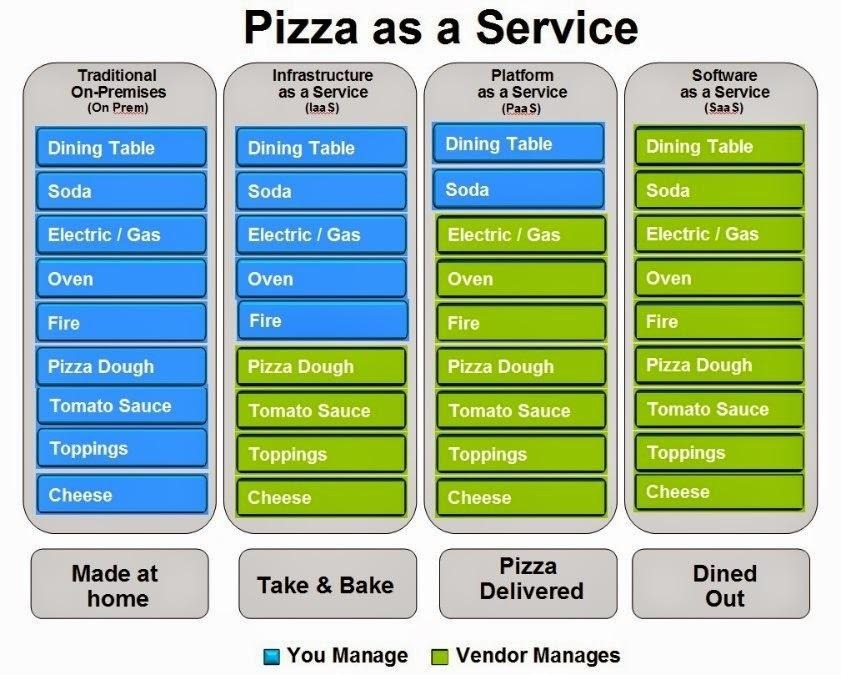
\includegraphics[width=\textwidth]{images/PizzaasaService.jpg}

				%\subsection*{approche envisagé}

					%\paragraph{cout}
					%\paragraph{consitence de la conf}
					%\paragraph{sécurité et privacité}
La frontière entre ces différents types d'infrastructure est parfois mince voire inexistante. Par exemple, la plate-forme web permettant de gérer ses infrastructures virtuelles chez n'importe quel fournisseur d'infrastructure comme un service\footnote{IaaS} n'est autre qu'un logiciel comme un service\footnote{SaaS}. De plus, les plate-formes IaaS fournissent généralement une solution de plate-forme comme une service\footnote{PaaS}. Google App Engine est une plate-forme PaaS fournie par Google et inclue dans l'offre Google Cloud, de la même façon Amazon Web Service propose Opswork.

De fait, ces concepts restent très théoriques et leurs implémentations ne sont jamais une vision absolue du concept. Il est donc important de bien comprendre ces services afin de définir le potentiel de chaque plate-forme d'hébergement et d'en exploiter au maximum les fonctionnalités.

%%%% miteux
Pour cela, nous utiliserons sept indicateurs permettant, selon mon expérience, de comparer la pertinence des différentes solutions présente sur le marché. C'est indicateurs sont les suivants:

\begin{description}

	\item[Sécurité]
		Contrôler l'accès aux ressources et aux données. Pouvoir garantir leur confidentialité.

	\item[Souveraineté]
		Posséder totalement ou partiellement ses ressources et données.

	\item[Flexibilité]
		Changer, se transformer, s'adapter aux besoins des utilisateurs.

	\item[Consistance]
		Garantir la configuration, les mises à jour.

	\item[Coût]
		Le nerf de la guerre qu'il faut savoir gérer pour ne pas ce retrouver sans électricité pour ses serveurs.

	\item[Barrières technologiques]
		Besoin en formation ou en personnel qualifié.

	\item[Pertinence technique]
		Puissance de calcul, mémoire, espace de stockage, outils innovants.

\end{description}
%%%%% miteux
%%%%%%%%%%%%% METHODOLOGIE %%%%%%%
Définir des indicateurs ne suffit pas à élaborer une stratégie. Les chiffres sont trop malléables pour pouvoir refléter la réalité. De plus, une projection linéaire ne peut être juste. Il faudrait au minimum l'indexer sur l'inflation afin d'appliquer une variance sur les projections pour que ces dernières soient en adéquation avec l'économie dans laquelle la structure évolue.

Il est tout même possible d'accorder 

Si tout se passe accordement au modèle, l’acquisition des utilisateurs est exponentielle. Les ressources nécessaires pour servir un volume de clients croissant de manière exponentielle est aussi théoriquement proportionnelle. Par extrapolation, les coûts suivent l’évolution


 même si les coûts sont faibles, ils ne sont toujours pas nuls. 


Il y a donc une limite mathématique à la réduction des coûts par les utilisateurs. C'est un palier annonçant la fin de la croissances des recettes et l'augmentation des coûts. Tant que les coûts par utilisateur baissent, la startup croît facilement. Nous pouvons reprendre, ici, le même principe que l’échange de monnaie ; étant donné que les marges réalisées grâce à la dépréciation d'une des monnaie par rapport à une autre, crée des profits. 
Prenons un exemple simple, lorsque je paie 800 euros pour obtenir 1000 dollars canadien, il est possible que quelques jours plus tard pour ces mêmes 1000 dollars je ne paie que 600 euros. Évidemment, je n'ai pas fait de recette, cependant j'ai limité les pertes. Pour pouvoir tirer profit d'un achat, il suffit de le revendre pour une somme supérieure au montant d'achats additionné aux frais. 
Pour cela, selon Adam Smith, nous n'avons qu'à attendre que la demande soit supérieure à l'offre \emph{La main invisible de l'économie} étant là pour réguler le marché, c'est à dire que selon lui, la loi du marché finit toujours par s'imposer et le réguler.

Si rien n'est fait, le taux peut devenir négatif alors chaque utilisateur deviendra une perte nette qui va s’accroire de manière exponentielle. A ce moment là, la seule chose restante à faire est de trouver des capitaux extrêmement rapidement afin d'éviter la faillite. 

Tant que les flux d'investissement ne se tarissent pas et que l'entreprise n'a pas fait faillite tout est encore possible.

%%%%%%%%%%%%%%%%%%%%%%%%%%%%%%%%%%%%


		% Méthodes habituellement utilisées pour une situation présentant des similitude
s
		\section{méthodes habituelles} % 5 pages

			\subsection{Les serveurs dans le placard ou dans la cave}

Cette solution permet d'être le seul et unique souverain de son infrastructure et de ses données. 

Néanmoins, il est impossible de fournir un service en haute disponibilité, car il suffit d'une panne de courant ou d'une terrible femme de ménage débrancheuse de serveurs pour que cela ne fonctionne plus. 
De plus, l'implémentation de mesure garantissant l'accès physique est impossible à mettre en place, à moins de posséder des moyens financiers importants ou de vivre préalablement dans un bunker. Ce qui ne serait peut être pas suffisant. Pour Kevin Mitnick\footnote{Hacker expert en ingénierie sociale, emprisonné à l'âge de 15 pour avoir pénétré des dizaines d'ordinateurs. Il a, d'ailleurs, passé 4 ans et 8 mois de sa peine en isolement. Selon Mitnick, les officiers de justice auraient convaincu le juge qu'il pourrait déclencher une guerre atomique en sifflant dans un téléphone.}, il n'existe pas de machine inaccessible, même un hôte isolé au fond d'un bunker est accessible car il ne suffit que de convaincre un garde de le brancher au réseau ou plus sobrement lui donner accés à la machine.

C'est une solution idéale pour un hobbyiste ou un groupe de passionnés car elle offre la pus grande liberté. Chacun met ce qu'il veut dans son placard. En revanche, les compétences nécessaires au maintient de l'infrastructure sont très importantes. Il faut savoir changer/réparer du matériel brisé ou usé mais ce n'est pas tout car tout est du fait de la personne gérant son infrastructure. 

Cette première méthode correspond à la représentation de l’imaginaire collectif des startups informatiques florissant dans les garages de la Sylicon Valley des années soixante-dix. 

%%%%% TABLEAU AVEC LES METRIQUE %%%%
\begin{center}
	\begin{tabular}{| l | c | }
		Souveraineté & Il est difficilement possible d'être plus souverain dans ce cas de figure. \\
	\end{tabular}
	\begin{tabular}{| l | c | }
		Sécurité & Obtenir un système sécurisé demande de grandes compétences, des moyens financiers importants, particulièrement pour la sécurisation des accès physiques. Une fois en place, cela peut devenir un véritable bastion technologique.\\
	\end{tabular}
	\begin{tabular}{| l | c | }
		Flexibilité & En un sens ces infrastructures ne peuvent répondre à une augmentation de demande trop importante. Commander et installer un serveur n'est pas instantané. \\
	\end{tabular}
	\begin{tabular}{| l | c | }
		Pertinence technique & C'est pertinent d'un point de vue personnel, non professionnel \\
	\end{tabular}
	\begin{tabular}{| l | c | }
		Coût & Difficilement chiffrable puisqu'il en vient de la responsabilité du constructeur de choisir ses matériaux, la taille de son serveur, etc.\\
	\end{tabular}
	\begin{tabular}{| l | c | }
		Barrières technologiques & Installer son propre placard à serveur \\
	\end{tabular}
\end{center}

			\subsection{Création de centre de données et cloud privé}

% c'est cher et chiant et si c'est pas chére c'pire
% Faut ce taper la sécurité physique + logiciel ainsi uqe l'entretiens des appareil réseaux et compute

% Véritable haute dispo extremement chere car min 2 datacenter pour PRA

% Ecologiquement difficile à chiffrer pas d'argus de la mort des non humains.

% Compétence +++++

% si compténce et pognons alors ça tue tout !!!!!!

% projection des coûts à 10 ans puissance pour de calcule

Calculer le coût exact de la construction et de l'exploitation d'un centre de données privée et au delà de mes compétences. Les facteurs de coûts son extrêmement nombreux. Beaucoup d'entreprises émettent une estimation inexacte de leur info-centre en raison de la fragmentation des centres de dépendance. Il est facile de négliger le poids d'un super-calculateur au moment de la construction du bâtiment. Ce qui arrive ensuite est simple: l'ordinateur, pesant plusieurs tonnes, traverse le sol pour aller décorer l'étage inférieur.

La mise en place d'une telle structure demande énormément de compétences aussi diverses que variées. Le comptable est tout aussi important que le directeur des services d'information car sans lui, il serait impossible d'exploiter financièrement la plateforme. 

En effet, il en va du constructeur d'élaborer toute l'infrastructure : de son système de refroidissement, à la sécurité du réseau en passant par l'achat, l'installation et la configuration du matériel\footnote{Tous les câbles doivent être branchés et si possible au bon endroit.}. 

S'il est dans les prérogative du centre de fournir un service de haute disponibilité, il sera nécessaire de construire deux sites physiquement distincts capables de se relayer en cas de panne afin d'offrir un plan de retour ou de non disruption de l'activité efficiente\footnote{L'efficience sera calculer en temps de présence disponibilité des ressources.}. 

%%%% REF data center Google
Il faut aussi prendre en compte l'impact du centre sur l'environnement. Ce dernier peut être négatif ou positif. Par exemple le data center de Google en Finlande récupère les eaux sales des villes environnantes. Elles sont ensuite réutilisées dans le système de refroidissement, traitées puis renvoyées potable dans le circuit de consommation ou rejetées \emph{froides} dans le golf d’Amina.

%%%%% TABLEAU AVEC LES METRIQUE %%%%
\begin{center}
	\begin{tabular}{| l | c | }
		Souveraineté &  L'exploitant étant en charge de l'infrastructure, il en a donc un contrôle total \\ 
	\end{tabular}
	\begin{tabular}{| l | c | }
		Sécurité & Mise en place de contrôle d’accès physique et bien entendu c'est à l'exploitant de le faire. \\
	\end{tabular}
	\begin{tabular}{| l | c | }
		Flexibilité & Les importants coûts d'exploitation demande une réflexion sur le long termes afin de le rentabiliser.  La flexibilité est donc très mauvaise.\\
	\end{tabular}
	\begin{tabular}{| l | c | }
		Pertinence technologique & C'est une solution adaptable aux grosses infrastructures mais qui, une fois installée, n'est pas toujours évolutive aisément. \\
	\end{tabular}
	\begin{tabular}{| l | c | }
		Coût & Ils sont très importants et complexes à évaluer car il faut prendre en compte des temps d'amortissement longs.\\
	\end{tabular}
	\begin{tabular}{| l | c | }
		Barrières technologiques & Le recours à de nombreux experts est nécessaire afin de mener à bien la création du centre de données. Une équipe d'ingénieurs et de techniciens sera, qui plus est, indispensable à la maintenance. \\
	\end{tabular}
\end{center}

			\subsection{Engin PaaS}

Il s'agit de plateforme d'hébergement virtualisée de nouvelle génération.  Bien que définie plus haut, je me permet de faire un petit rappel sur le PaaS. Ces structures proposent d'héberger les sources de votre logiciel, le client se déchargeant de la gestion des systèmes.
%Incompatible dans l'état d'happyBox à cause de la persistance des données

Les ressources proposées sont souvent dispendieuses et sont soumises à une limitation sur le nombres de langages implémenté par la plateforme.

Ce sont des plateformes offrant le meilleur taux d'évolutivité et de réponse pour utilisateurs. La plateforme fournira exactement les ressources dont l'application à besoin.

Le véritable aspect des ce type de service est l'absence de pertinence de donnée autrement que dans une base de donnée.

Finalement l'externalisation peut entraîner une dépendance technologique néfaste et des situations où l'hébergeur de donnée pourrait prendre en otage le client.

%%%%% TABLEAU AVEC LES METRIQUE %%%%
\begin{center}
	\begin{tabular}{| l | c | }
		Souveraineté & Faible voire nulle\\
	\end{tabular}
	\begin{tabular}{| l | c | }
		Sécurité & Gérer de manière logicielle.\\
	\end{tabular}
	\begin{tabular}{| l | c | }
		Flexibilité & C'est l'évolution incarnée; augmenter ou réduire la puissance de distribution peut même être géré par la plateforme.\\
	\end{tabular}
	\begin{tabular}{| l | c | }
		Pertinence technique & Permet de répondre à une énorme demande très rapidement.\\
	\end{tabular}
	\begin{tabular}{| l | c | }
		Coût & Proportionnel à la consommation de ressources.\\
	\end{tabular}
	\begin{tabular}{| l | c | }
		Barrières technologiques &  extrêmement faibles\\
	\end{tabular}
\end{center}


			\subsection{Consistance des infrastructures et méthode de déploiement}

La lois de Moore institue que la puissance de calcul des systèmes d'information double tous les six mois mais que ses administrateurs ne semblent pas être sujets à cette multiplication spontanée. Du coup, les infrastructures accueillent de plus en plus d'hôtes au sein de leur ferme mais le personnel n'augmente pas toujours à la même célérité. 

Des outils de gestion de configuration distribués ont vu le jour dans le but de répondre à la forte hausse de la demande. Ils ce composent souvent d'un tiers local sur la machine à configurer et un tiers distant gérant la distribution des configurations.

Ils permettent de garantir une uniformité\footnote{consistance} de déploiement et de configuration par unité de sens défini par le développeur. Ceci permet d'éviter les longues séances de recherche d'incident au milieu d'un centre de données.

Cette gestion des configurations est alliée à un outil de gestion de code sources afin de proposer une solution intégrant déploiement applicatif et mise à jour de logiciel. Plus de détails seront apportés à ce sujet dans la partie suivante.

%Mais y a moyen de moyenner et on vois ça aprés. cf provisionning

		% Exposé des décisions prise et des interventions menée par le stagiare pour résoudre le problème
\section{Une infrastructure à batis dans le nuage.}	 % 15 pages

		% Petite intro bien sympa présentant la méthodes suivis:
		% 	- stat
		% 	- action
		% 	- stat
		% 	- action
		% 	- sieste
		% 	cf linux bibl

	\subsection{création de l'infra} % 5 pages

				% faire plusieurs itération faut vendre du vent et tomber des pages d
				% parler de la limite mathématique de l'équation
\paragraph{}
Une de mes premières missions au sein de DOM Element Inc a été de définir les besoins en hébergement de la solution. Pour cela, il a fallu commencer par définir exactement le fonctionnement de HappyBox CMS.

\begin{center}
	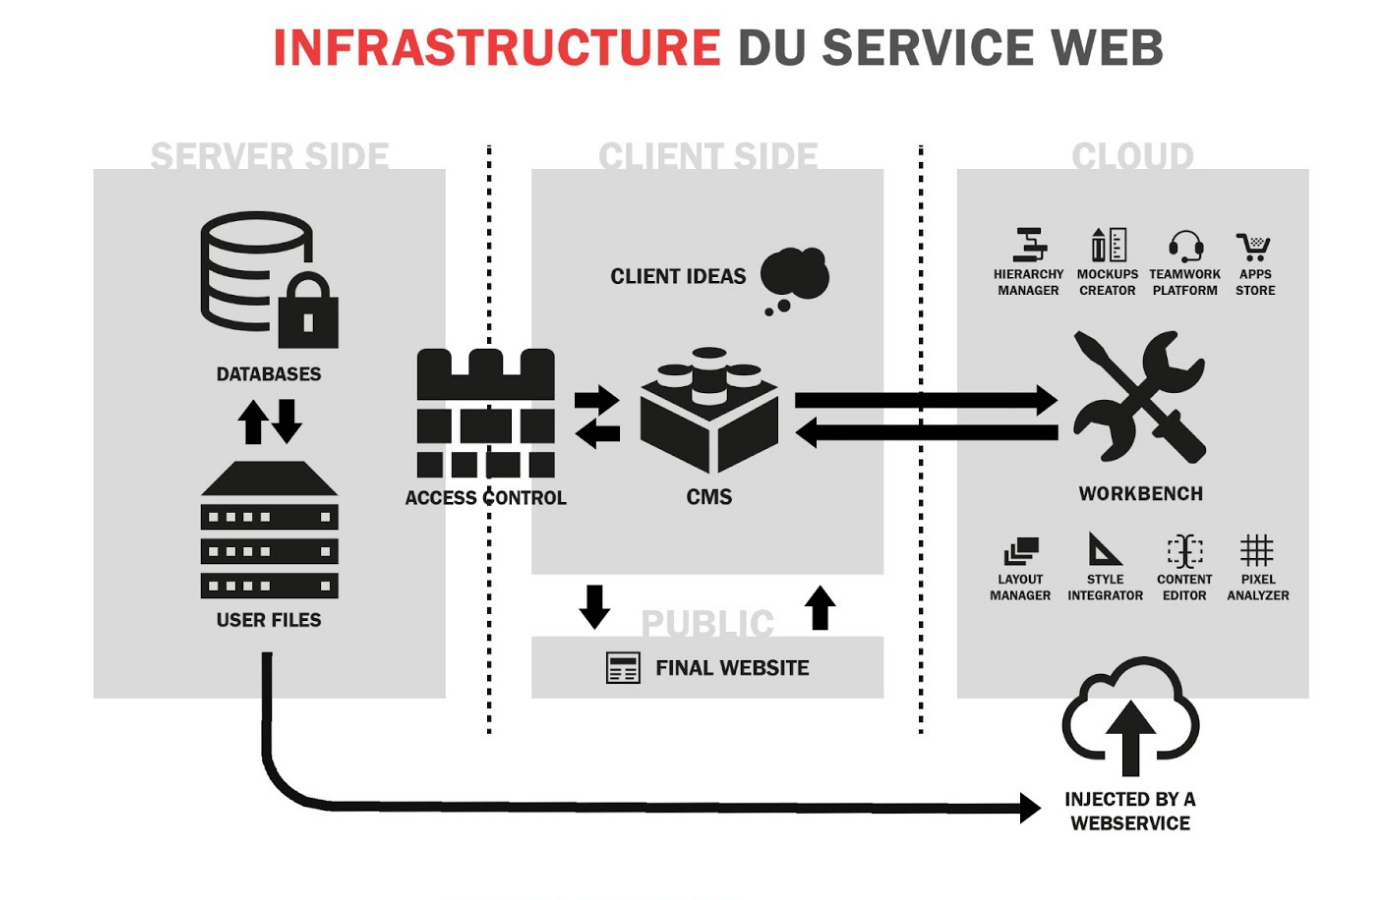
\includegraphics[width=\textwidth]{images/media/fonctionnementHB.png}
\end{center}
\paragraph{}
L'architecture minimale, nécessaire au fonctionnement de HappyBox CMS, nécessite en premier lieu un serveur web pour héberger les données des utilisateurs. Une base de donnée gére les permissions et permet de coordonner l'ensemble des opérations. Le dernier élément est un serveur permettant d’héberger l'API DOM Element Inc.. 
\paragraph{}
Chaque élément a put être installé sur des serveurs séparés, mais il est aussi possible de tous les gérer sur un seul hôte bien que cette solution ne nous est pas paru pertinente. En effet, en terme d'évolutivité, cette solution lie les clients à une instance virtuelle qui est gérée localement. 
Si les ressources de ce dernier viennent à manquer, il faudra recréer un nouvel hôte, ré-installer et configurer chaque service. En cas d'erreur sur ce serveur, le rendant inaccessible, les clients hébergés dessus n'auront plus accès au service.
Il a été décidé, avant mon arrivée, de séparer ces éléments en trois tiers distincts: serveurs client, API et bases de données.
\paragraph{}
La gestion des bases de données est faite au sein du service \emph{Relational Database Services} proposé par Amazon Web Services et propose un moteur de base de données relationnel hébergé. Cette solution nous a permis de simplifier la gestion de l’infrastructure en externalisant les opérations de maintien des bases bien que cette assertion ne soit pas toujours juste aux vues des erreurs que nous avons rencontrer. En juillet, ce dernier a entraîné un arrêt de service pour une durée de 2 jours. Après investigation, nous avons découvert que l'instance de base de données avait été redémarré par l'agent AWS et n'avait pas réussi à redémarrer. En conséquence, les sites créés par les utilisateurs étaient toujours accessibles mais l'inscription et l'accès au logiciel HappyBox était impossible.
Ce genre d'erreur ne génère une alerte que dans l'interface de gestion du service sur le site de AWS. Sur ce même site ce genre d'interface sont pléthoriques, rendant le diagnostique parfois long et difficile. J'ai donc configuré des alertes envoyées par courriel qui m'indiquaient en temps réel les erreurs. Ce qui a grandement facilité la recherche d'erreurs par la suite.
\paragraph{}
Une fois la structure générale en place, je me suis concentré sur les aspects spécifiques à chaque élément. 
J'ai donc décidé d'organiser mon travail selon deux grands axes: entretien et surveillance de l’infrastructure, déploiement et configuration du logiciel au sein de l'infrastructure. 

\subsection{Déploiement et configuration}

Comme nous l'avons vu précédemment HappyBox est un logiciel composé de trois éléments distincts. On peu ajouter à cela la gestion des serveurs de nom de domaine\footnote{DNS, Domain Name Services} qui est une composante fondamentale car chaque site créé par un utilisateur est relié à une adresse internet de type \emph{nomDeLaPage.happyboxcms.me} ou composé à partir d'un domaine qui appartient à l'utilisateur\footnote{Domaine qu'il peut acheter directement au sein de l'interface ou ajouter s'il en est déjà propriétaire.}.
\paragraph{}
La première chose à mettre en place est une API DOM Element afin de pouvoir manipuler les utilisateurs et coordonner le service. Je n'ai fait que peu de chose en ce qui concerne son déploiement et sa configuration qui est assez simple car il s'agit simplement d'un site web capable de répondre à des requêtes faites par le client. Ce processus est transparent pour l'utilisateur. 
\paragraph{}
Il a fallu ensuite faire le choix du serveur web permettant de servir les clients. Nous avons choisi d'utiliser le logiciel Nginx. À proprement parler, Nginx n'est pas un serveur web. Il s'agit d'un logiciel de proxy dont la fonction primaire n'est pas de permettre l'affichage de site web mais de réguler le trafic allant d'un point à un autre et qui offre les possibilité d'un serveur web traditionnel. Il est plus performant que les autres logiciels de ce type en terme de service de contenu statique. Couplé à un module d’interprétation php, il offre toutes les possibilités d'un serveur web avec un pic de performance dans la distribution de contenu statique. En revanche, son architecture modulaire\footnote{Nginx est constitué d'un binaire capable de gérer le trafic entrant et de renvoyer uniquement du contenu statique. Des modules offrant de nouvelles fonctionnalités peuvent ensuite être ajoutées afin de n'installer que ce dont on a besoin et de ne pas gâcher des ressources pour des services inutiles.} le rend plus complexe à installer qu'un serveur web de type apache car il faut compiler le cœur avec ses modules ou installer un paquet logiciel et un autre pour chaque module que l'on doit configurer séparément.
\paragraph{}
Dans mon cas, il a été obligatoire d'installer Nginx avec une douzaine de modules\footnote{installer séparément.} permettant la gestion du langage php, du cache et bien d'autre. Une fois l'installation terminée, il a fallu configurer les serveurs Nginx ainsi que ses modules en éditant des fichiers de configuration dans des formats non unifiés et dépendants du module. J'ai également, installer d'autres services, comme un serveur ftp\footnote{Service de transfert de fichier}, un agent de mail enfin, j'ai créé les dossiers pour accueillir HappyBox CMS. 
\paragraph{}
Une fois environnement prêt à accueillir le logiciel, le déploiement peut commencer. Il se fait par le biais de deux dépôts de source: un pour la partie utilisateur visible sur internet et une seconde servant à la maintenance par un système de message. 
\subparagraph{}
De plus, les sources du logiciel n'étaient pas centralisé. Il est possible que la mauvaise version soit déployée par erreur.   
\subparagraph{}
C'est un processus long et capable de générer des erreurs aussi hétéroclites que nombreuses car chaque élément est un facteur d'erreur potentielle. De plus, d'un serveur à l'autre, il est possible que les versions des logiciels utilisées ainsi que leurs fichiers de configuration soient différents. La recherche d'erreur est une fois encore complexifiée.
\paragraph{}
J'ai donc proposé que nous changions de méthode de déploiement afin d'essayer d'obtenir un parc uniforme donc consistent. J'ai donc proposé l'utilisation de deux service: un pour la gestion des configurations et un autre pour la gestion de la version du code source.  
\paragraph{}
En ce qui concerne la gestion de version du code source le choix à était le suivant: conserver la gouvernance et la souveraineté de l'hébergement des sources gràce au logiciel gitlab ou recourir à un service en ligne github ou bitbucket. Au finale, nous avons décidé de conserver les sources au sein de l'infrastructure. J'ai donc installer sur un serveur gitlab et configuré le service. Ce dernier offre tout les avantages de la gestion des source via git\footnote{Système de gestion des sources décentralisé créer utiliser pour le maintiens du noyau linux.} allié à une interface graphique intuitive.
\paragraph{}
Une fois les sources accessibles par version et non par clef usb qui transite dans le bureau, je me suis intéressé au différent système de gestion de configuration distribuée. La solution qui m'a paru la plus viable est le service \emph{Opswork} proposé dans le cadre d'Amazon Web Services. Il propose la gestion de l'infrastructure via une pile logiciel composée de couches logiques et définie par unité de sens. Il s'agit de l'implémentation du logiciel \emph{chef} dans les services AWS. En plus de la gestion de configuration, Opswork propose un service de déploiement type \emph{PaaS}, un outil de surveillance, un autre de gestion de charge horizontale.
\paragraph{}
Opswork est donc l'implémentation de chef dans le service AWS. L'utilisation d'Opswork requiert la création de livre de recette ou cookbook. Ces livres de recette sont développés dans le langage de programmation rubi qu'il m'a fallu apprendre et maîtriser. Ils sont composés de gabarit qui sont la base de nos fichiers de configuration, de fichier d’attribut qui permettent de stocker des valeurs accessibles n'importe où dans livre de recette. Ces dernières définissent une liste d'action à exécuter.
\paragraph{}
Le développement ainsi que le maintien des cookbook ne sont pas une mince affaire et demande de la méthode car la configuration déployée sera la même sur l'intégralité du parc. C'est à dire qu'une configuration rendant l'instance inaccessible sera appliquée à tous les hôtes utilisant le livre de recette déficient. 
\paragraph{}
Ma méthode est la suivante: Dans un premier temps définir les différentes unités de sens qui seront nos livre de recette. J'ai choisi d'en créer 3 principaux qui définiront le fonctionnement de déploiement. 
\subparagraph{}
Le premier permet de préparer l’hôte de manière générique. Ce livre de recette n'est pas lié à l'architecture de HappyBox mais est constitué d'un ensemble de configuration et d'action exécutée avant le déploiement à proprement parler. On y trouve les réglages généraux, par exemple la configuration de la langue et du temps. La création des utilisateurs administratifs ainsi que leurs accès distants via ssh. L'installation et la configuration de l’éditeur de texte vim et quelques autres petites configurations de moindre importance.
\subparagraph{}
Le second correspond à l'installation et à la configuration du serveur web et de ses composantes ainsi que d'un agent de transfert de courriel. C'est à partir de cet instant que la gestion de configuration devient importante car elle permet de garantir que peu importe le moment où l'on vérifiera le serveur, il y aura toujours la même version et la même configuration sur toutes les instances. 
\subparagraph{}
Le dernier crée l'architecture de dossiers nécessaires au fonctionnement d'HappyBox, configure les tâches planifiées puis déploie et configure HappyBox CMS en fonction de la version souhaitée. Il sert aussi à mettre à jour l'application grâce à des recettes offrant le choix du type d'installation voulue: développement, production ou compatibilité avec l'ancienne version du logiciel\footnote{Certains utilisateurs ont des projets créés et non compatibles avec les versions plus récentes.}.
\paragraph{}
La mise en place d'Opswork a eu un impact significatif dans l'installation et la mise à jour logiciel. Avant cela, il fallait prévoir une après-midi entière pour déployer une nouvelle version voir plus en cas de problèmes. Maintenant, il suffit de dire à l'agent de mettre à jour ou d'installer la version souhaitée sur les serveurs concernés, ce qui est un gain de temps non négligeable. De plus, la résolution des erreurs est beaucoup plus rapide car une erreur ne concernant qu'un seul serveur ne peu être liée à un des éléments présente dans les livres de recette. L'erreur est sur toutes les machines virtuelles et sa résolution dans la recette concernée réparera toutes les instances de manière simultanée. Par extrapolation: une erreur isolée sur un serveur n'est pas due aux livre de recette, ce qui exclue donc d'office une partie des pistes d'investigation.
\begin{center}
	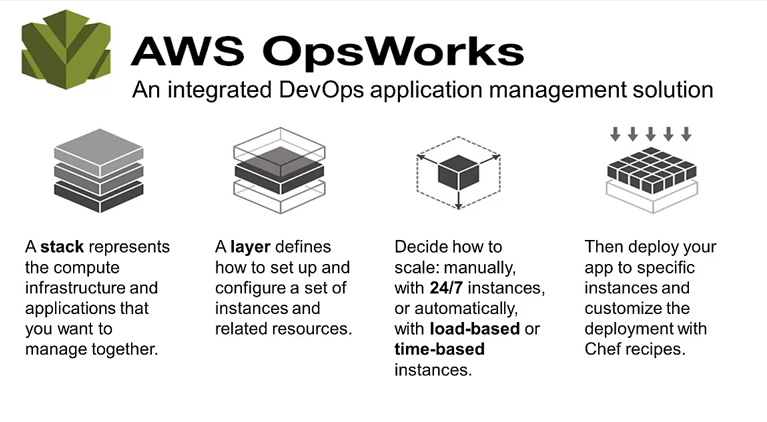
\includegraphics[width=\textwidth]{images/opswork.png}
\end{center}

%%%%% JIRA %%%%%
\paragraph{}
Après avoir mis en place une structure pour gérer le logiciel. Nous avons pensé qu'il serait judicieux de mettre en place un outil nous permettant d'organiser le travail. Il m'a incombé de chercher et tester la meilleure solution. Après plusieurs essais avec différentes plateformes, nous avons décidé d'utiliser Jira de la compagnie Atlassian. 
\subparagraph{}
Ce logiciel permet de gérer les tâches de tout le monde de manière centralisé via une interface web différent projet et les droits d’accès. Dans ces projet, il est possible de créer et d'assigner des tâches aux membres. Cela permet de mieux coordonner et de suivre le travail de tous. Il fonctionne par un système de tickets. Le service étant un logiciel SaaS, il nous a suffi de payer l'abonnement pour y accéder.


%%%%% L'horreur des volumes EBS
\paragraph{}
Vint le jour de cette magnifique idée : un volume de données par utilisateurs afin de les rendre mobiles et indépendants. J'ai donc proposé l'idée à Danny et Guillaume qui m'ont donné leur aval afin de me lancer dans ce chantier de grande ampleur. 
\subparagraph{}
Amazon Web Service proposant une interface de programmation dans différents langages, j'ai développé des script permettant de créer  des volumes de données automatiquement lors de la création de compte. Il était ensuite attaché à l'instance et monté afin de pouvoir accueillir au mieux les données des utilisateurs. 
J'ai testé la solution sur une instance à part afin de ne pas interagir directement sur des serveurs en production. À la suite de ces tests, qui ont semblé concluant, nous avons procédé à l'intégration au sein du service lors de l'ajout d'un hôte.
\subparagraph{}
Peu de temps après, j'ai pu constaté l'erreur que cela a été. En effet, le temps de traitement des nouveaux comptes a commencé à renvoyer des erreurs ne créant pas convenablement les volumes qui restaient verrouillés dans un état de création infinie ne pouvant alors être attachés aux instances. Un mécanisme de secours permettant de stocker temporairement les données utilisateurs dans un dossier sur le serveur, a permis d'éviter les interruptions de service dues aux erreurs. 
\subparagraph{}
Avec le nombre croissant de volumes, les opérations de sauvegarde et de récupération se sont vues sensiblement complexifiées. De plus, la migration des utilisateurs entre les différentes instances est devenue une opération complexe car chaque volume devait être attaché et monté correctement sur le nouvel hôte. Il faut encore préciser qu'au moment de la décision un paramètre essentiel à été oublié: pour augmenter la taille d'un volume, il faut le supprimer et en recréer un de taille supérieure. Sachant que l'offre d'HappyBox propose la possibilité, moyennant finance, d'agrandir l'espace d'un utilisateur. Cette solution était vouée à mourir. 
\subparagraph{}
Après investigation je me suis rendu compte que parfois l'interface de programmation d'Amazon Web Services annoncée comme étant synchrone ne l'était pas. En effet, une action peut renvoyer un état achevé alors que ce n'est pas encore le cas. Les opérations suivantes ne peuvent donc pas s'exécuter correctement et sont susceptibles de mettre en échec l'intégralité de l'instance.

\subparagraph{}
Finalement, j'ai pris la décision de changer de méthode lors de la migration du serveur de production. La nouvelle méthode de stockage des données se base à l'heure actuelle sur un espace de stockage commun à tous les utilisateurs de la même instance. Cela a rendu possible la conservation du cloisonnement et l'implémentation des mécaniques permettant d'agrandir et de réduire la taille d'un espace de stockage virtuel aisément. La migration d'un serveur s'en trouve simplifiée car il suffit de connecter le volume partagé sur le nouvel hôte et d'y déclarer ses nouveaux utilisateurs. La sauvegarde est elle aussi simplifiée étant donné qu'au moment de sauvegarder un volume par utilisateur, on sauvegarde le volume partagé des utilisateurs.


\subsection{Entretiens et surveillance de l'infrastructure}

Cet axe de travail est sûrement celui qui a occupé la majeure partie de mon temps et ralenti considérablement la mise en place de nouveauté au sein de l'infrastructure. 

% MAJ
\paragraph{}
Il s'agissait, ici, de tester les nouvelles versions des logiciels utilisés sur les serveurs dans un environnement cloisonné afin d'éviter une mauvaise synergie ou une version comprenant des erreurs capables de mettre en échec un hôte ou un service nécessaire au bon fonctionnement d'HappyBox CMS.

La méthodologie appliquée pour cela a été la suivante: 
Dans un premier temps, un nouvel hôte identique à ses pères, grâce au gestionnaire de configuration, est déployé. La mise a jour a été faite manuellement sur l'hôte de test afin d'en décrire le processus et de pouvoir l'ajouter aux livres de recette existants. 
Ensuite, le logiciel est testé afin de voir si tout est fonctionnel tant du côté de la machine que du logiciel. 

\subparagraph{}
Ce test est composé de deux étapes: une première sur le système et une seconde en ligne sur l'interface d'HappyBox. J'en ai, pour ce fait, conçu plusieurs qui m'ont permis de tester les services qui exécutent des actions courantes telles que créer un utilisateur, modifier l'espace de stockage, ou encore le réduire, communiquer avec la base de données, etc.
Les fichiers d’enregistrement, ou fichiers de log, sont ensuite analysés grâce au logiciel \emph{Logstash} qui permet de trier et d'inventorier des fichiers d'enregistrement selon des règles définies à l'avance.

La seconde consiste à aller sur l'interface de l'instance de test et d'utiliser le logiciel afin de voir si tout fonctionne correctement.


\subsection{Calcul du coût d'un utilisateur}

Il m'a aussi été demandé de calculer le coût exact d'un utilisateur gratuit sur HappyBox CMS. 
